\documentclass{article}

\usepackage{graphicx}  % For including images if needed
\usepackage{hyperref}  % For hyperlinks
\usepackage{amsmath}   % For math symbols if needed
\usepackage{enumitem}  % For better list formatting
\usepackage{placeins}
\usepackage{booktabs}
\usepackage{url}
\usepackage{float}
\usepackage{subcaption}

\usepackage[style=numeric, sorting=ydnt]{biblatex}
\addbibresource{references.bib}

\title{Machine Learning - Final Project }
\author{Michael Dadush 206917908 \\ Shay Gali 315202242}
\date{March 2025}


\begin{document}

\maketitle


\section{Introduction}

Gender and age classification in not controlled settings shows big challenges due to many imaging conditions and problems in the data. In our project, we deal with these issues by making a framework that includes data exploration, preprocessing, feature extraction, model training, and checking performance. All our code and implementation details can be seen on our github repository \cite{github_repo}.

We start our project with deep data exploration to understand main characteristics and challenges of Adience Benchmark dataset. This first analysis is in the \texttt{data\_exploration.ipynb} notebook, which shows data distribution, imaging conditions, and what preprocessing we need. You can see notebook and follow our exploration by visiting \href{https://github.com/ShayGali/VisAge/blob/main/data_exploration.ipynb}{data\_exploration.ipynb}.

This introduction part prepare for next detailed discussions about challenges and the strategies we use to overcome them, making sure we have good approach to solve the gender and age classification problem.

After data exploration, we try several models we learn in our course, like Softmax regression, Support Vector Machines (SVM), and other machine learning methods. To make feature representation better, we try different image transformations like grayscale and RGB. Also, we use Principal Component Analysis (PCA) for dimensionality reduction, so we can check if compact representations improve classification performance. The classical models we implement are in the \texttt{old\_models} directory on GitHub: \href{https://github.com/ShayGali/VisAge/tree/main/old_models}{old\_models folder}.

After we check individual models, we want to combine our findings by using multiple models trained on different image representations. We develop two pipelines: one for grayscale images and another for RGB images. These approaches are in separate notebooks:
\begin{itemize}
    \item \textbf{Grayscale Models:} We train various models on grayscale images and check their performance. The complete implementation is in \href{https://github.com/ShayGali/VisAge/blob/main/grayscale_models.ipynb}{grayscale\_models.ipynb}.
    \item \textbf{RGB Models:} We do similar experiments on RGB images, comparing if color information give better classification accuracy. This notebook is at \href{https://github.com/ShayGali/VisAge/blob/main/rgb_models.ipynb}{rgb\_models.ipynb}.
\end{itemize}

With models trained and checked, we answer key research questions about gender and age classification. Our analysis and findings for first question are in \href{https://github.com/ShayGali/VisAge/blob/main/questions/q1.ipynb}{q1.ipynb}.

To show practical use of our model, we create real-time camera application that predicts gender and age from live video. This application, in the \texttt{camera-viewer-app} folder, shows how model works in real situations. The source code for this application is at \href{https://github.com/ShayGali/VisAge/tree/main/camera-viewer-app}{camera-viewer-app}.

\section{Description of the Database}
We chose to work with the Adience Benchmark dataset for Gender and Age Classification\cite{adience_dataset}. This dataset has real-world images of faces, which makes it good for testing different machine learning methods. The dataset includes:

\subsection*{Labels in Dataset}
The dataset provides many labels for each data point, we used the followinglabels for our analysis:
\begin{itemize}[leftmargin=1.6cm]
    \item \textbf{gender}: Male / Female
    \item \textbf{age}: The dataset categorizes images into the following age ranges: 0--2 years, 4--6 years, 8--12 years, 15--20 years, 25--32 years, 38--43 years, 48--53 years, 60 and above
    \item \textbf{user\_id, face\_id, original\_image}: These labels are used to identify the image and the person in the image.
    \item The dataset includes more labels that we did not use in our analysis, but we explain what each label means in the dataset in the {data exploration notebook}\cite{github_repo}.
\end{itemize}
\section{Analysis of the Database}

\subsection{Data Exploration and Preprocessing}
When we explore the Adience Benchmark dataset, we find several important characteristics and preprocessing needs:

\begin{enumerate}
    \item \textbf{Duplicate Directories}: At first look, we find two directories with name "faces" that contain image files. After we check more, we see that one directory (with 40 files) is just small part of the other one (with 168 files). We choose the big directory with all 168 user folders for our work.
    
    \item \textbf{Data Organization}: The dataset is organize in 5-fold cross-validation way, with data in files named "fold\_0\_data.txt" to "fold\_4\_data.txt". We use Folds 0-3 (with 15,554 entries) for training, and fold 4 (with 3,816 entries) for testing, so totally we have 19,370 entries before we do preprocessing.
    
    \item \textbf{Missing Values}: The original dataset have some entries with missing values. After we remove these entries, we get 18,551 complete records, which mean only small part (about 4.2\%) of data is incomplete.
\end{enumerate}


\subsection{Age Classification Standardization}
One of big challenges when we work with Adience dataset was the not consistent representation of age information:

\begin{enumerate}
    \item \textbf{Overlapping Age Ranges}: Dataset had many overlapping age ranges that we need to fix:
    \begin{itemize}
        \item The ranges (38, 42), (38, 43), and (38, 48) we merge into (38, 43) based on frequency analysis (46, 2293, and 6 instances)
        \item One weird (8, 23) age range with only one instance we remove
        \item The less common (27, 32) range (77 instances) we merge into more frequent (25, 32) range (4,953 instances)
    \end{itemize}
    
    \item \textbf{Single Age Values}: Dataset had 1,094 entries with single age values not ranges. We map these to right age ranges based on how close they are:
    \begin{itemize}
        \item Ages 2, 3 → (0, 2), (4, 6)
        \item Age 13 → (8, 12)
        \item Ages 22, 23, 29, 34 → (25, 32)
        \item Ages 35, 36, 42 → (38, 43)
        \item Ages 45, 46, 55 → (48, 53)
        \item Ages 57, 58 → (60, 100)
    \end{itemize}
    
    This standardization give us consistent set of eight age ranges: (0, 2), (4, 6), (8, 12), (15, 20), (25, 32), (38, 43), (48, 53), and (60, 100).
\end{enumerate}

\subsection{Gender Distribution Analysis}
\begin{itemize}
    \item Female: 9,332 samples (50.3\%)
    \item Male: 9,216 samples (49.7\%)
\end{itemize}


\begin{figure}[H]
    \centering
    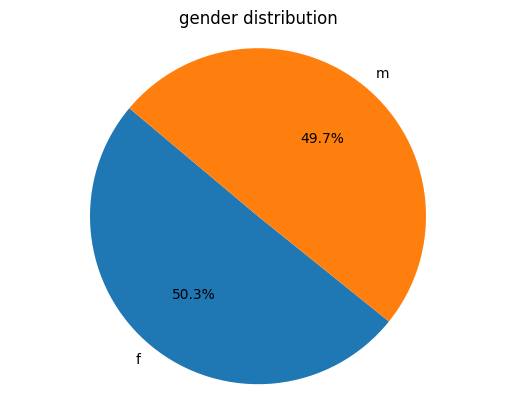
\includegraphics[width=0.8\textwidth]{assets/gender distribution.png}
    \caption{Gender Distribution in the Adience Benchmark Dataset}
\end{figure}



\subsection{Age Distribution Analysis}

After standardization, the age distribution across the eight defined ranges was:

\begin{itemize}
    \item (0, 2): 2,491 samples (13.4\%)
    \item (4, 6): 2,158 samples (11.6\%)
    \item (8, 12): 2,287 samples (12.3\%)
    \item (15, 20): 1,642 samples (8.9\%)
    \item (25, 32): 5,391 samples (29.1\%) 
    \item (38, 43): 2,695 samples (14.5\%)
    \item (48, 53): 990 samples (5.3\%)
    \item (60, 100): 896 samples (4.8\%) 
\end{itemize}

\begin{figure}[H]
    \centering
    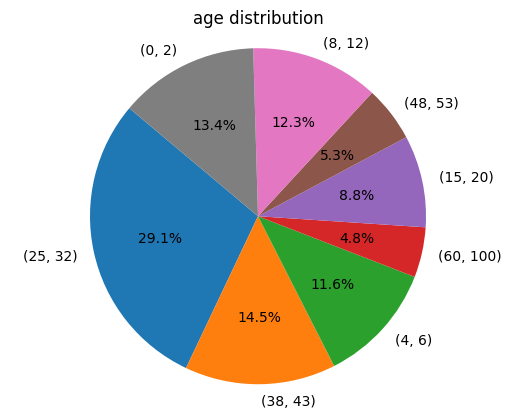
\includegraphics[width=0.8\textwidth]{assets/age distribution.png}
    \caption{Age Distribution in the Adience Benchmark Dataset}
\end{figure}


\subsection{Combined Age-Gender Analysis}

The intersection of age and gender categories revealed interesting patterns:

\begin{itemize}
    \item The (25, 32) age range showed the highest representation for both genders, with 3,026 female and 2,363 male samples.
    \item Gender distribution within age groups varied significantly:
    \begin{itemize}
        \item (0, 2): 684 female vs. 1,807 male 
        \item (8, 12): 1,353 female vs. 932 male
        \item (25, 32): 3,026 female vs. 2,363 male
        \item (48, 53): 458 female vs. 532 male
        \item (60, 100): 428 female vs. 467 male
    \end{itemize}
\end{itemize}

\paragraph{}
This combined analysis provides valuable insights into potential intersectional biases that might emerge during model training, particularly in the youngest age group where gender assignment was artificial rather than determined from image features.


\begin{figure}[H]
    \centering
    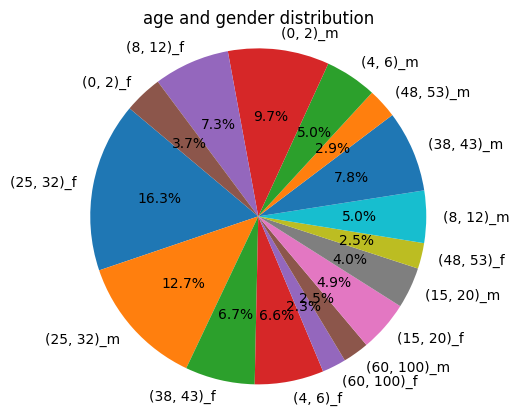
\includegraphics[width=0.8\textwidth]{assets/age and gender distribution.png}
    \caption{Combined Age and Gender Distribution in the Adience Benchmark Dataset}
\end{figure}

\subsection{Data Partitioning and Integrity}
To make sure we have good evaluation way, we split the dataset into three parts:

\begin{itemize}
    \item Training set: 11,850 samples (63.9\%)
    \item Validation set: 2,963 samples (16.0\%)
    \item Test set: 3,729 samples (20.1\%)
\end{itemize}

We check very carefully that no overlap exist between these sets by checking if any image identifiers and face IDs appear in more than one set. This check confirm complete separation, which is very important for fair performance evaluation.


\newpage
\section*{Tools used in the project}

The following tools and techniques were used in this project :

\begin{itemize}
    \item Softmax
    \item SVM
    \item Random Forest
    \item Adaboost
    \item KNN
    \item Multi-layer Perceptron (MLP)
    \item ResNet50- as feature extractor and as a model
    \item PCA - as a feature extractor
\end{itemize}

\newpage
\section{Training Methodology}

\subsection{Feature Extraction}

For most of our models, we used pre-trained networks to extract meaningful features from face images rather than training directly on raw pixel values.

\begin{itemize}
    \item \textbf{ResNet50 Feature Extraction}: We utilized the ResNet50 architecture pre-trained on ImageNet to transform raw images into 2048-dimensional feature vectors. This was implemented for both RGB and grayscale processing pipelines.
    
    \item \textbf{Image Preprocessing}: Before feature extraction, images were resized to 224×224 pixels and normalized according to ImageNet statistics. For grayscale processing, single-channel images were duplicated across three channels to match ResNet50's input requirements.
    
    \item \textbf{Batch Processing}: To manage memory efficiently, images were processed in batches of 64, with separate feature sets created for training, validation, and test partitions.
\end{itemize}

We also try PCA as a feature extraction method, but the results were not as good as the ResNet50 feature extraction method, so we decided to use the ResNet50 feature extraction method for our models.


\subsection{Data Preprocessing}
After feature extraction, we did several preprocessing steps to prepare the data for model training:

\begin{itemize}
    \item \textbf{Feature Standardization}: We standardize features to have zero mean and unit variance using scikit-learn's StandardScaler, which we fit on training set and apply to validation and test sets.
    
    \item \textbf{Label Encoding}: We encode the combined age and gender labels (e.g., "(25, 32)\_f" for female in 25-32 age range) into numeric indices using LabelEncoder.
    
    \item \textbf{Class Weights}: To fix class imbalance in dataset, we compute balanced class weights that are inverse to class frequencies, so minority classes get right attention during training.
\end{itemize}

\subsection{Model Training Approaches}

We train two parallel sets of models—one with RGB features and another with grayscale features—to compare which is better:

\begin{itemize}
    \item \textbf{Traditional Machine Learning}: For Softmax (Logistic Regression), SVM, Random Forest, AdaBoost, and KNN models, we use scikit-learn implementations.
    
    \item \textbf{Neural Network Models}: For MLP model, we implement architectures in TensorFlow with dropout and batch normalization to stop overfitting. Training use Adam optimizer with categorical cross-entropy loss and early stopping based on validation set performance.
    
    \item \textbf{CNN Training}: These models we train directly on image data instead of extracted features.
\end{itemize}


\subsection{Evaluation Methodology}
To ensure robust evaluation of model performance:

\begin{itemize}
    \item \textbf{Metrics}: We primarily used accuracy as our evaluation metric, calculated on both training and test sets to assess overfitting.
    
    \item \textbf{Confusion Matrix Analysis}: We analyzed confusion matrices to understand the types of errors made by each model, particularly focusing on whether errors occurred between adjacent age groups or across gender boundaries.
    
    \item \textbf{Cross-Comparison}: Performance was compared across RGB and grayscale processing pipelines to determine whether color information provided meaningful advantages.
\end{itemize}

All models were saved after training for later deployment and testing in real-world scenarios, which informed our analysis of practical applications detailed in the research questions section.


\newpage
\section{Model Performance}
\subsection{Grayscale scores}

\subsubsection{Grayscale Model Training and Testing Accuracy}
Table \ref{tab:Grayscale scores} summarizes the accuracy results of different models on the dataset using grayscale image.

\begin{table}[htbp]
    \centering
    \begin{tabular}{lccc}
        \toprule
        Model & Train Accuracy & Test Accuracy & Notes \\
        \toprule
        Softmax & 0.7095 & 0.3135 & \parbox[t]{6cm}{most of the error in the confusion matrix was in the adjacent age group.} \\
        \midrule
        SVM & 0.2046 & 0.1781 & \parbox[t]{6cm}{the model predict for the most of the data to 25-32 age group, and the gender was female.} \\
        \midrule
        Random Forest & 0.7730 & 0.3167 & \parbox[t]{6cm}{the model predict for the most of the data to 25-32 age group, but he got the gender right.} \\
        \midrule
        AdaBoost & 0.3467 & 0.2650 & \parbox[t]{6cm}{the  have berrly predict classes that he dont have a lot of data.} \\
        \midrule
        K-NN (k=1) & 0.9998 & 0.2202 & \parbox[t]{6cm}{we can see the overfitting -  the train accuracy is very high, but the test accuracy is very low.} \\
        \midrule
        K-NN (k=3) & 0.7525 & 0.2258 & \parbox[t]{6cm}{we can see start of overfitting - most of the error in the confusion matrix was near the (25,32) age group - the majority class.}\\
        \midrule
        K-NN (k=5) & 0.7001 & 0.2314 & \parbox[t]{6cm}{the over fitting is less significant}\\
        \midrule
        K-NN (k=7) & 0.6631 & 0.2422 & \parbox[t]{6cm}{the over fitting is less significant} \\
        \midrule
        K-NN (k=9) & 0.6331 & 0.2440 &  \parbox[t]{6cm}{the over fitting is less significant} \\
        \midrule
        MLP & 0.7521 & 0.3229 & \parbox[t]{6cm}{the model with the less overfitting, and when the model got wrong predictions, it was not by much (the most of the error in the confusion matrix was in the adjacent age group).} \\
        \midrule
        CNN & 0.4371 & 0.3153 & \parbox[t]{6cm}{this model have overffiting - it predict most of the data to the (25,32) age group.} \\
        \bottomrule
    \end{tabular}
    \caption{Train and Test Accuracy of Various Models with grayscale method}
    \label{tab:Grayscale scores}
\end{table}

\subsubsection{Grayscale Model Confusion Matrices}
Here are confusion matrices for grayscale models, they show where model predictions are right (on diagonal) and where they are wrong (not on diagonal).

\begin{figure}[H]
    \centering
    \begin{subfigure}[b]{0.48\textwidth}
        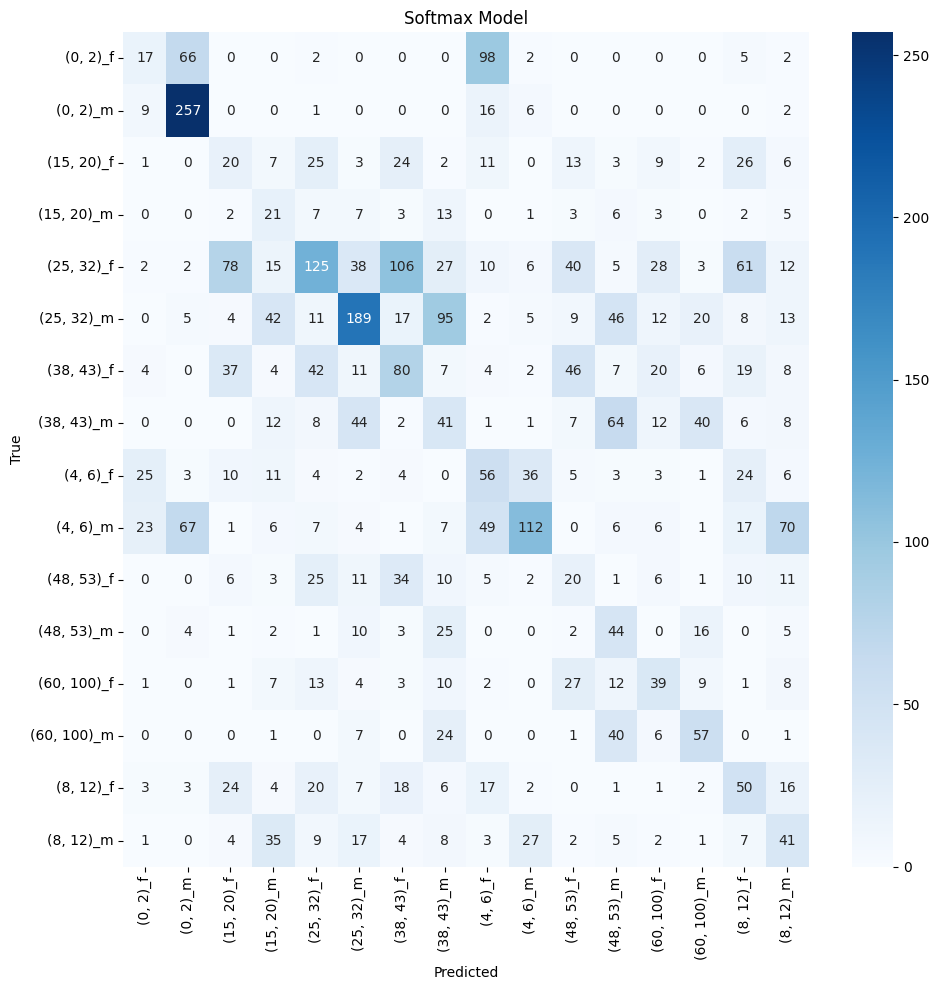
\includegraphics[width=\textwidth]{assets/confusion_matrix/grayscale/Softmax Model.png}
        \caption{Softmax}
    \end{subfigure}
    \hfill
    \begin{subfigure}[b]{0.48\textwidth}
        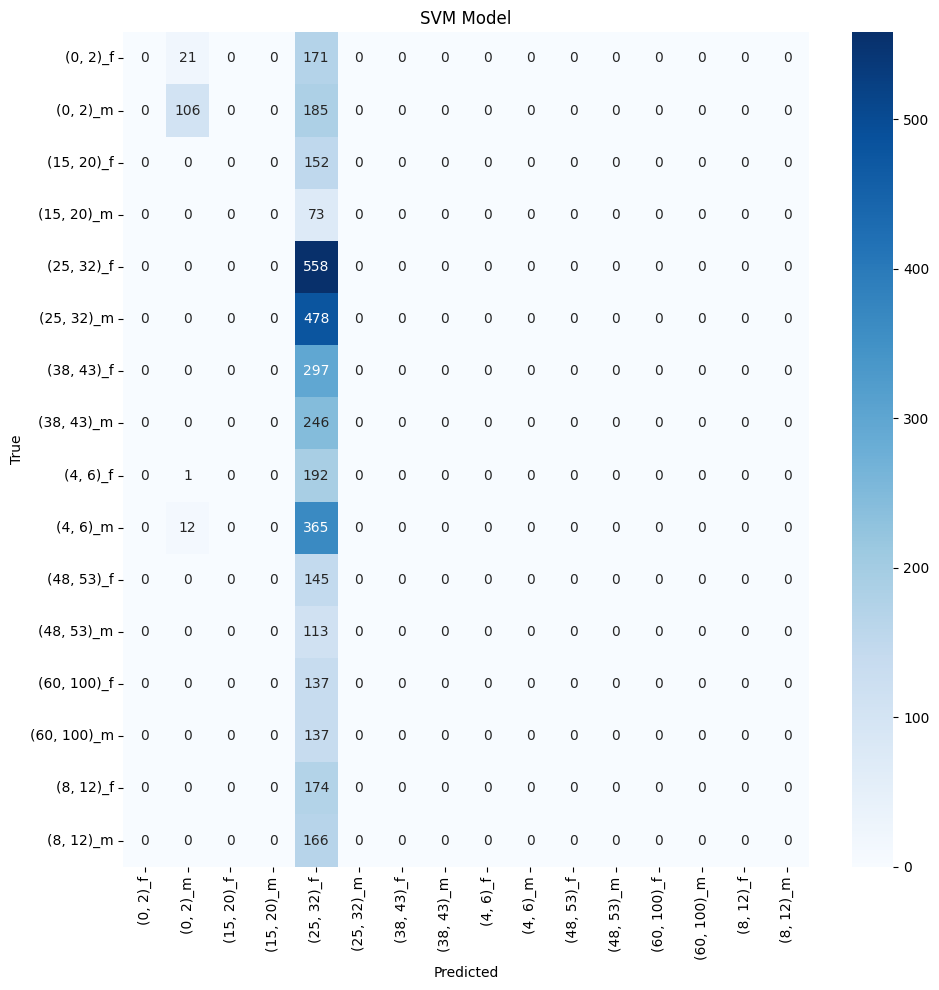
\includegraphics[width=\textwidth]{assets/confusion_matrix/grayscale/SVM Model.png}
        \caption{SVM}
    \end{subfigure}
    \caption{Confusion matrices for Softmax and SVM models (grayscale)}
    \label{fig:grayscale_confusion_matrices_1}
\end{figure}

\begin{figure}[H]
    \centering
    \begin{subfigure}[b]{0.48\textwidth}
        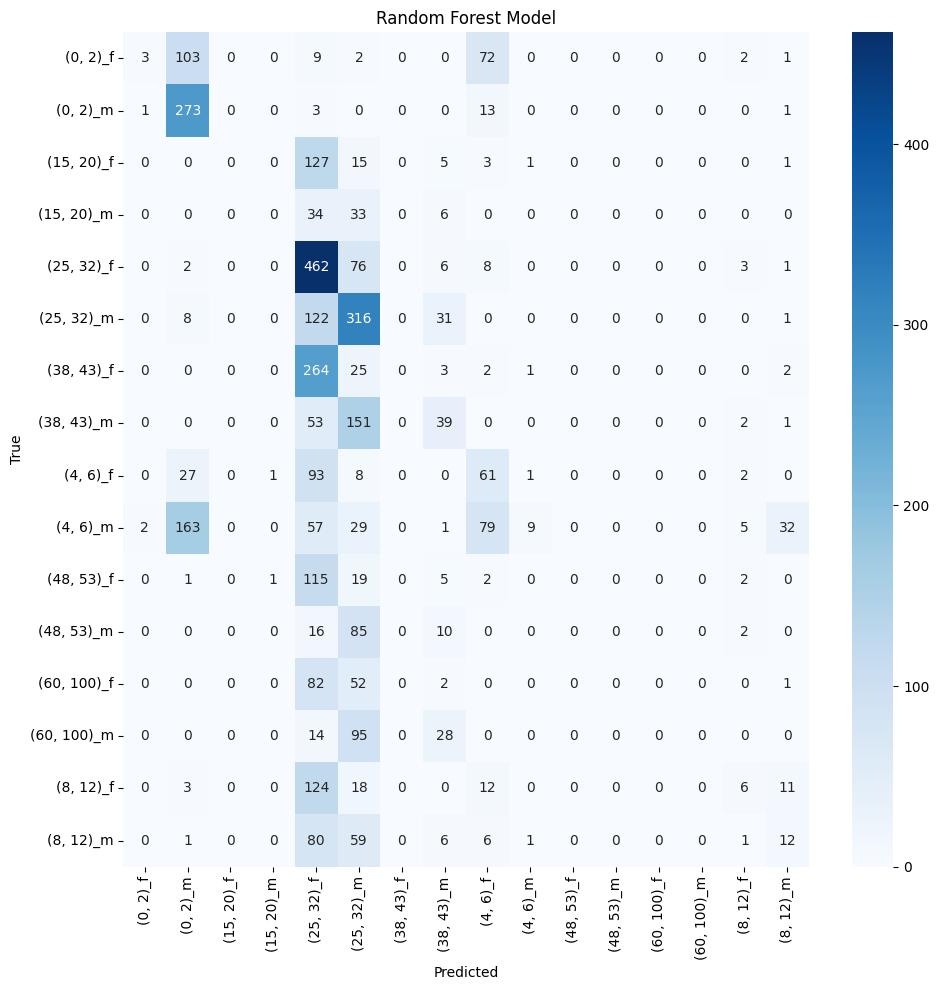
\includegraphics[width=\textwidth]{assets/confusion_matrix/grayscale/RF Model.png}
        \caption{Random Forest}
    \end{subfigure}
    \hfill
    \begin{subfigure}[b]{0.48\textwidth}
        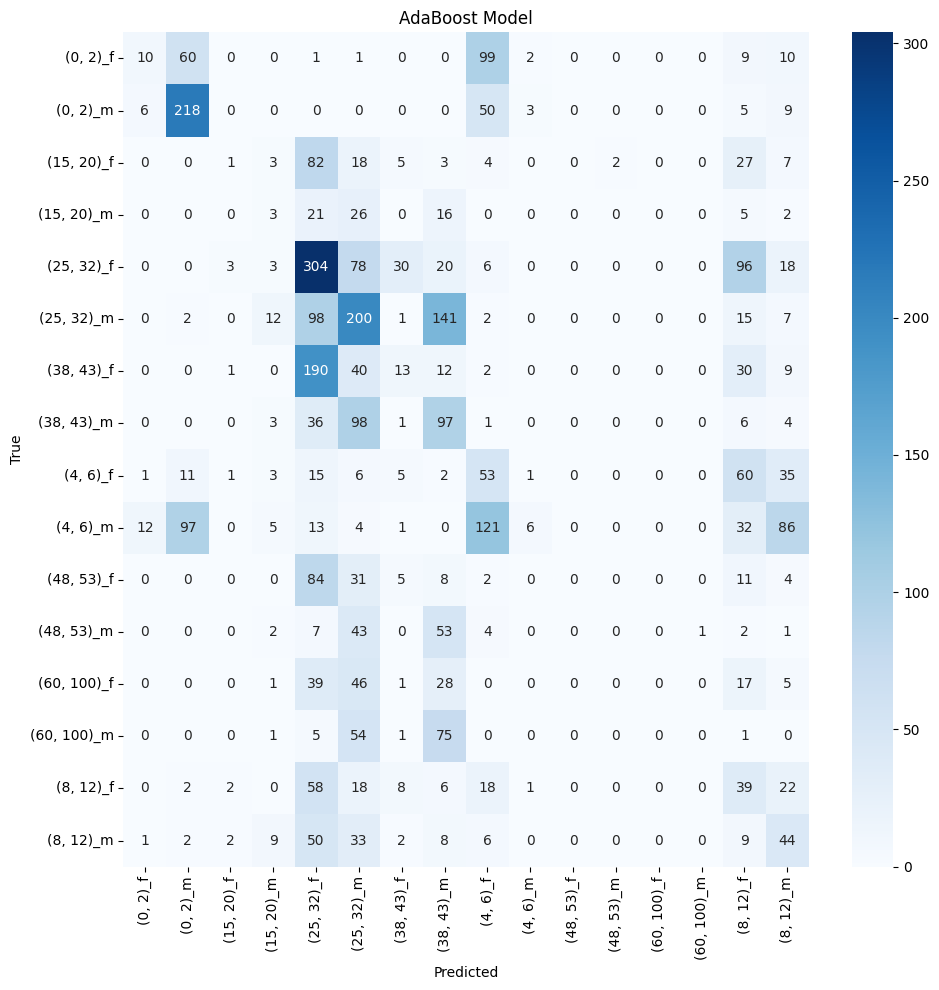
\includegraphics[width=\textwidth]{assets/confusion_matrix/grayscale/AdaBoost Model.png}
        \caption{AdaBoost}
    \end{subfigure}
    \caption{Confusion matrices for Random Forest and AdaBoost models (grayscale)}
    \label{fig:grayscale_confusion_matrices_2}
\end{figure}

\begin{figure}[H]
    \centering
    \begin{subfigure}[b]{0.48\textwidth}
        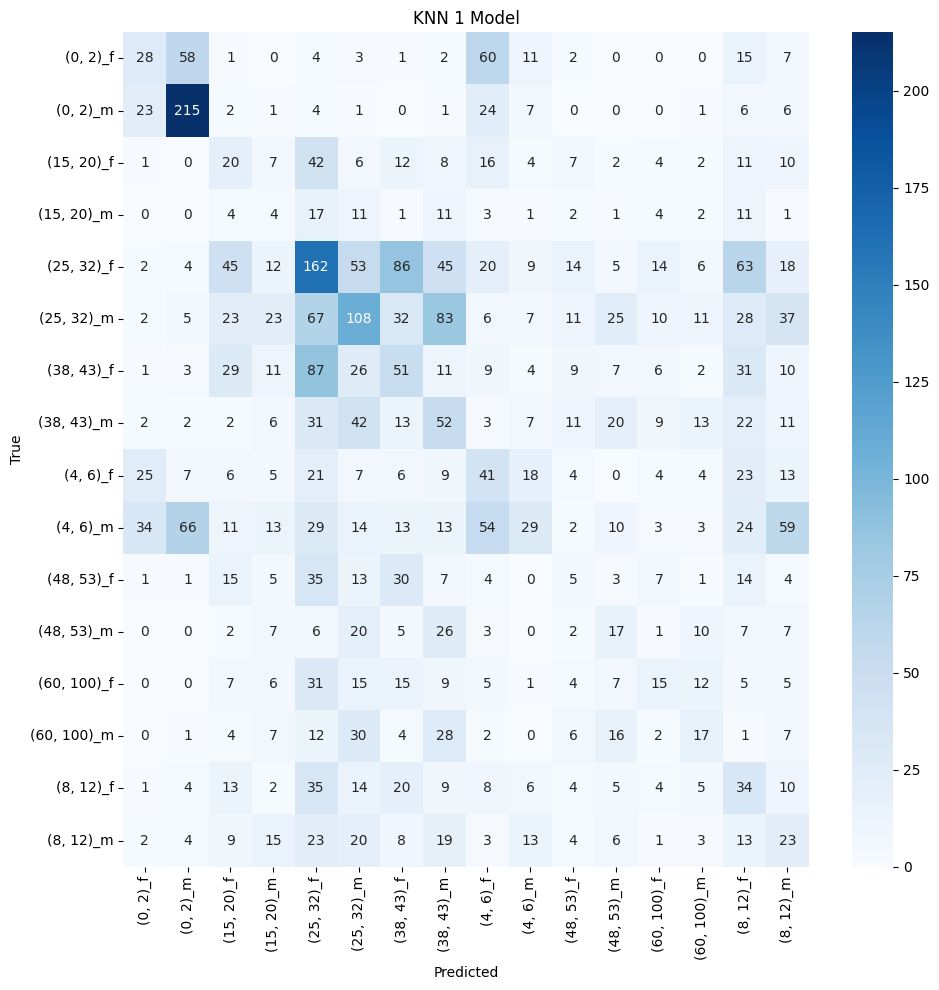
\includegraphics[width=\textwidth]{assets/confusion_matrix/grayscale/KNN1.png}
        \caption{KNN (k=1)}
    \end{subfigure}
    \hfill
    \begin{subfigure}[b]{0.48\textwidth}
        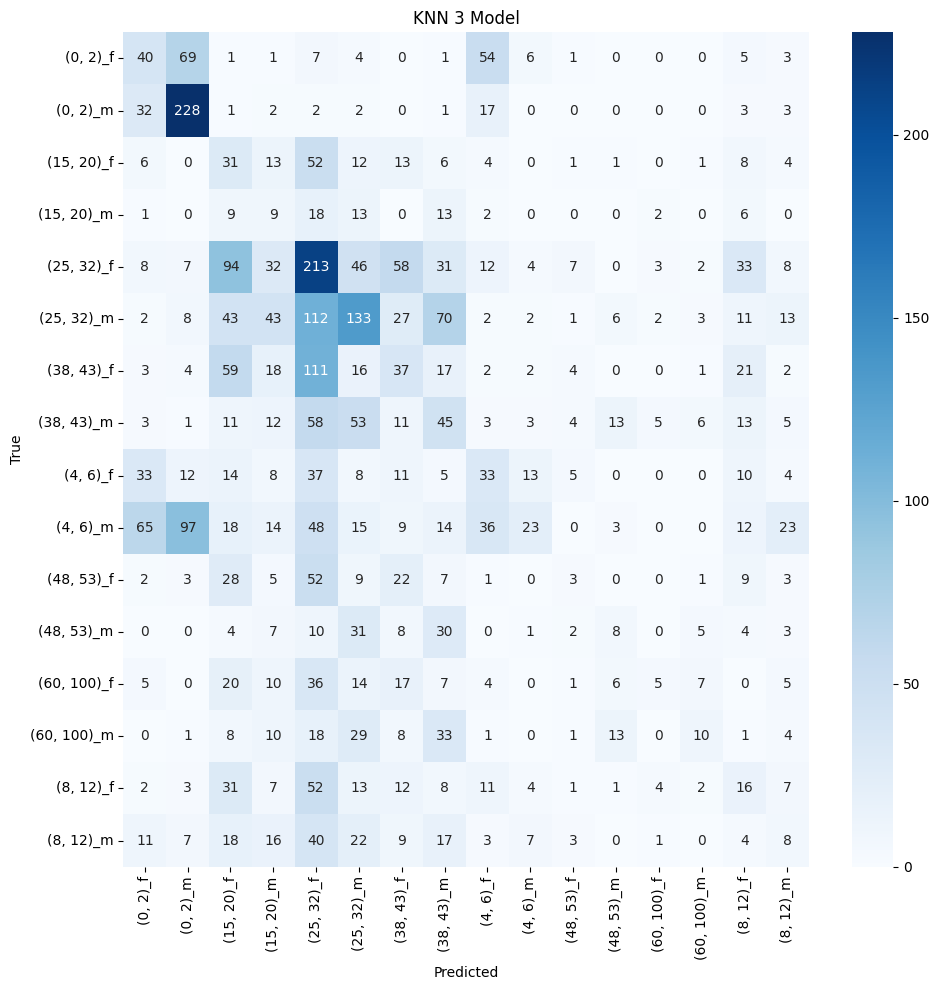
\includegraphics[width=\textwidth]{assets/confusion_matrix/grayscale/KNN3.png}
        \caption{KNN (k=3)}
    \end{subfigure}
    \caption{Confusion matrices for KNN models with k=1 and k=3 (grayscale)}
    \label{fig:grayscale_confusion_matrices_3}
\end{figure}

\begin{figure}[H]
    \centering
    \begin{subfigure}[b]{0.48\textwidth}
        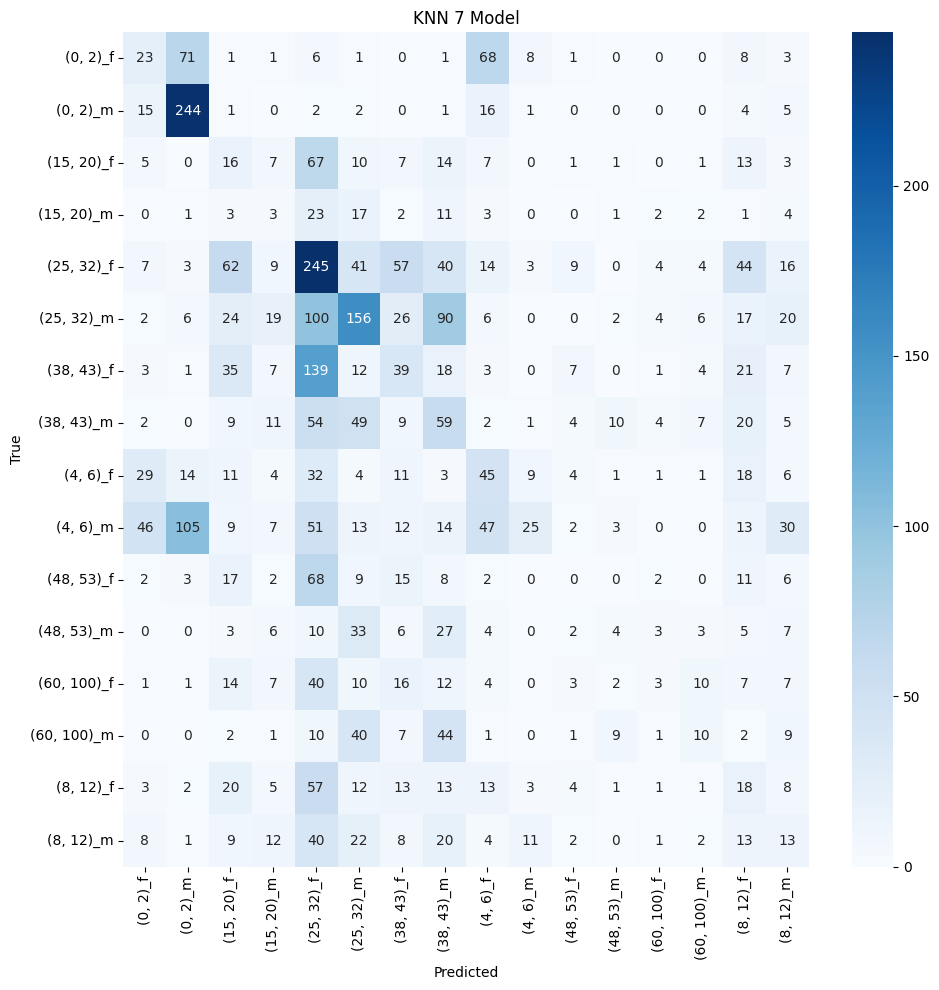
\includegraphics[width=\textwidth]{assets/confusion_matrix/grayscale/KNN7.png}
        \caption{KNN (k=7)}
    \end{subfigure}
    \hfill
    \begin{subfigure}[b]{0.48\textwidth}
        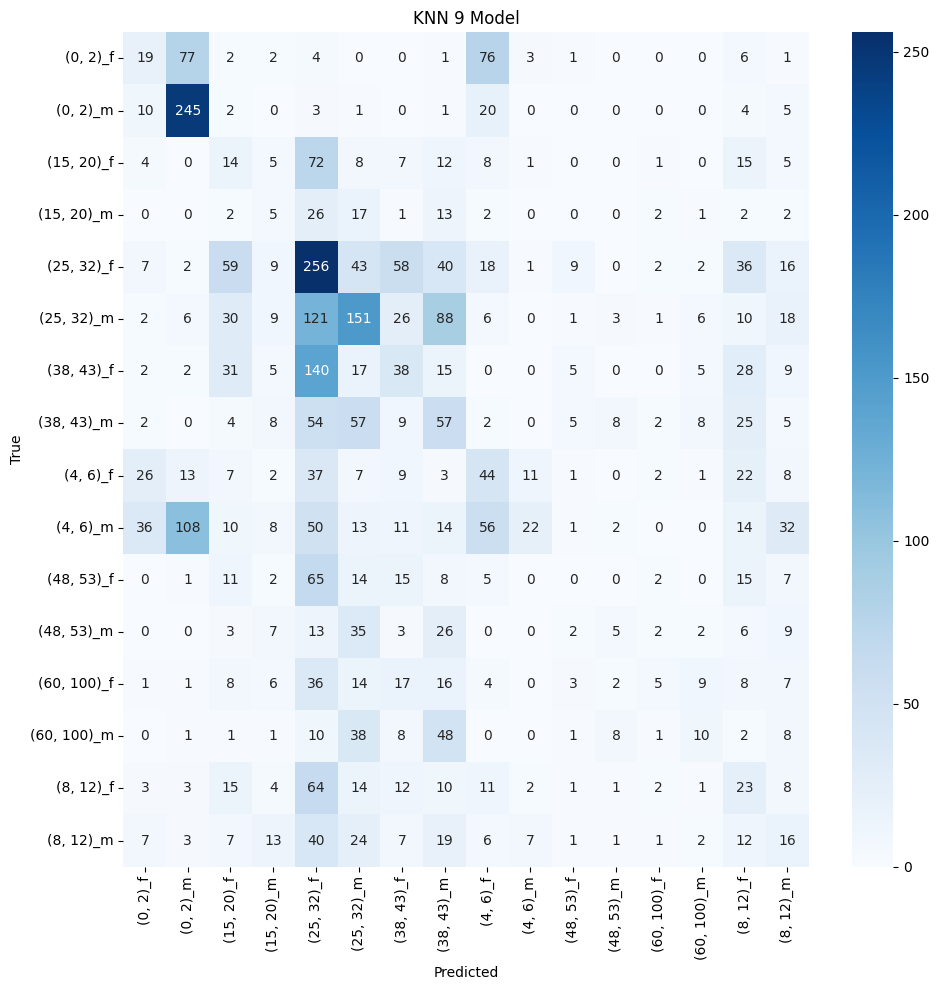
\includegraphics[width=\textwidth]{assets/confusion_matrix/grayscale/KNN9.png}
        \caption{KNN (k=9)}
    \end{subfigure}
    \caption{Confusion matrices for KNN models with k=7 and k=9 (grayscale)}
    \label{fig:grayscale_confusion_matrices_4}
\end{figure}

\begin{figure}[H]
    \centering
    \begin{subfigure}[b]{0.48\textwidth}
        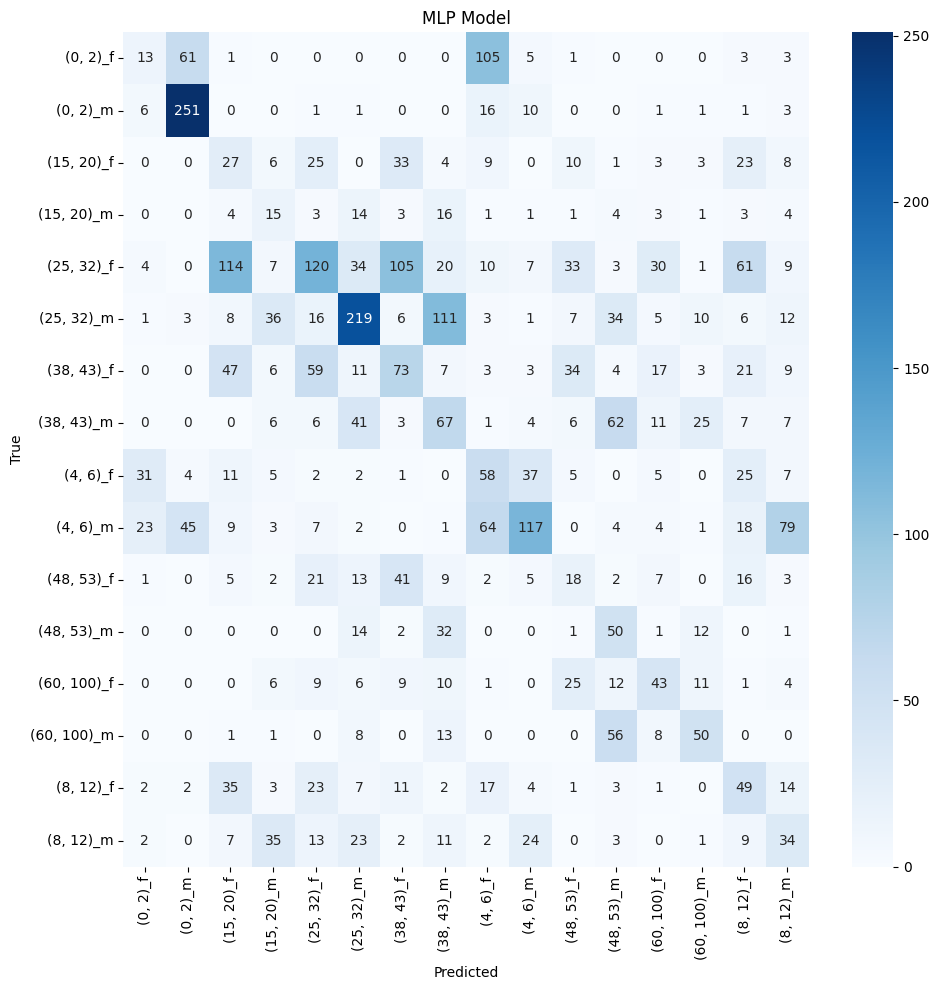
\includegraphics[width=\textwidth]{assets/confusion_matrix/grayscale/MLP.png}
        \caption{MLP}
    \end{subfigure}
    \hfill
    \begin{subfigure}[b]{0.48\textwidth}
        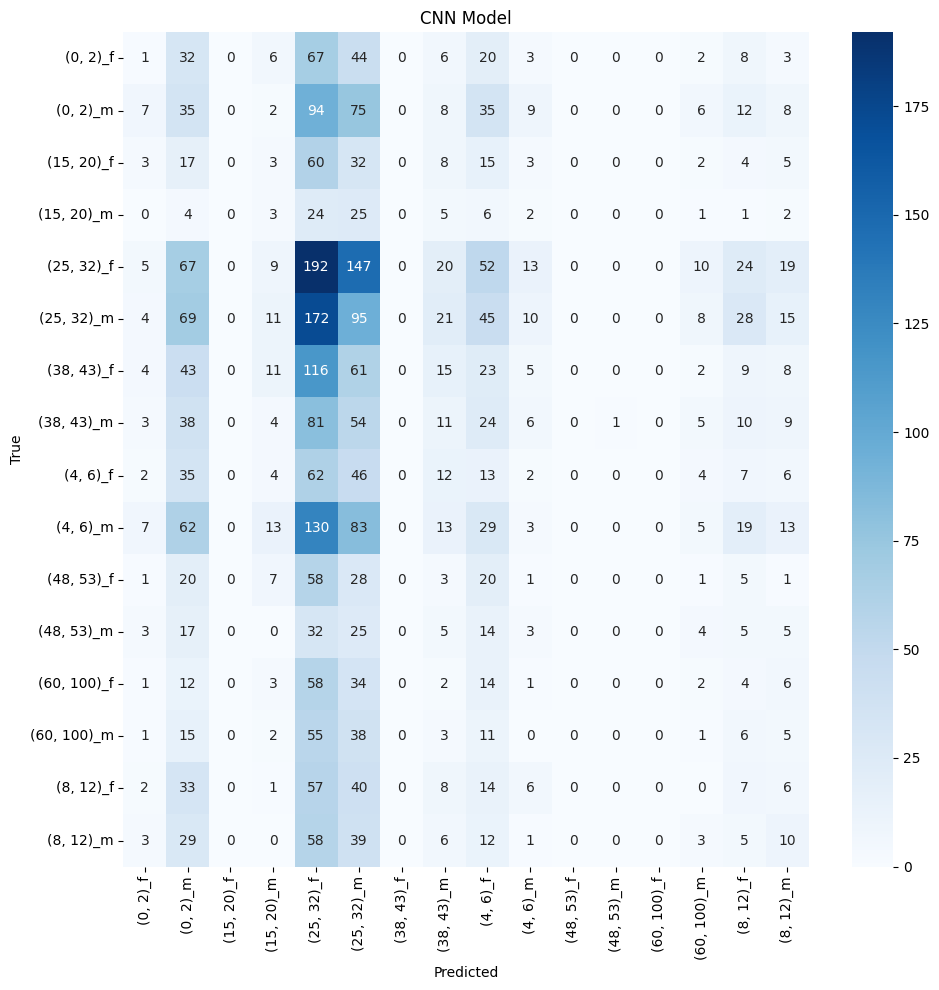
\includegraphics[width=\textwidth]{assets/confusion_matrix/grayscale/CNN.png}
        \caption{CNN}
    \end{subfigure}
    \caption{Confusion matrices for MLP and CNN models (grayscale)}
    \label{fig:grayscale_confusion_matrices_5}
\end{figure}

\begin{figure}[H]
    \centering
    \begin{subfigure}[b]{0.48\textwidth}
        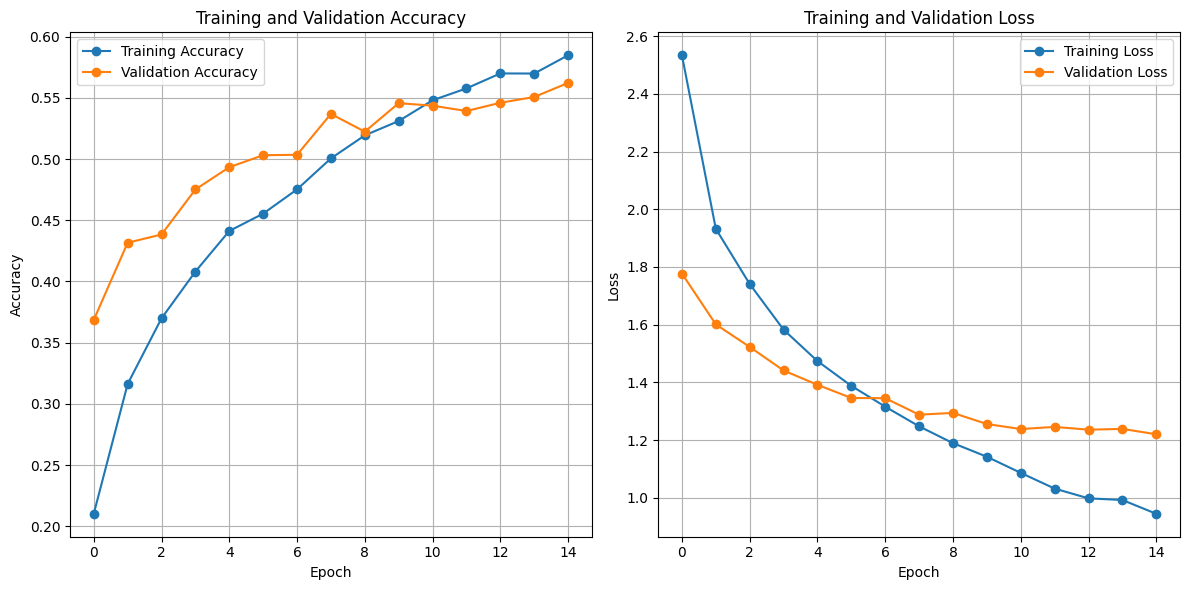
\includegraphics[width=\textwidth]{assets/confusion_matrix/grayscale/MLP_history.png}
        \caption{MLP training history}
    \end{subfigure}
    \hfill
    \begin{subfigure}[b]{0.48\textwidth}
        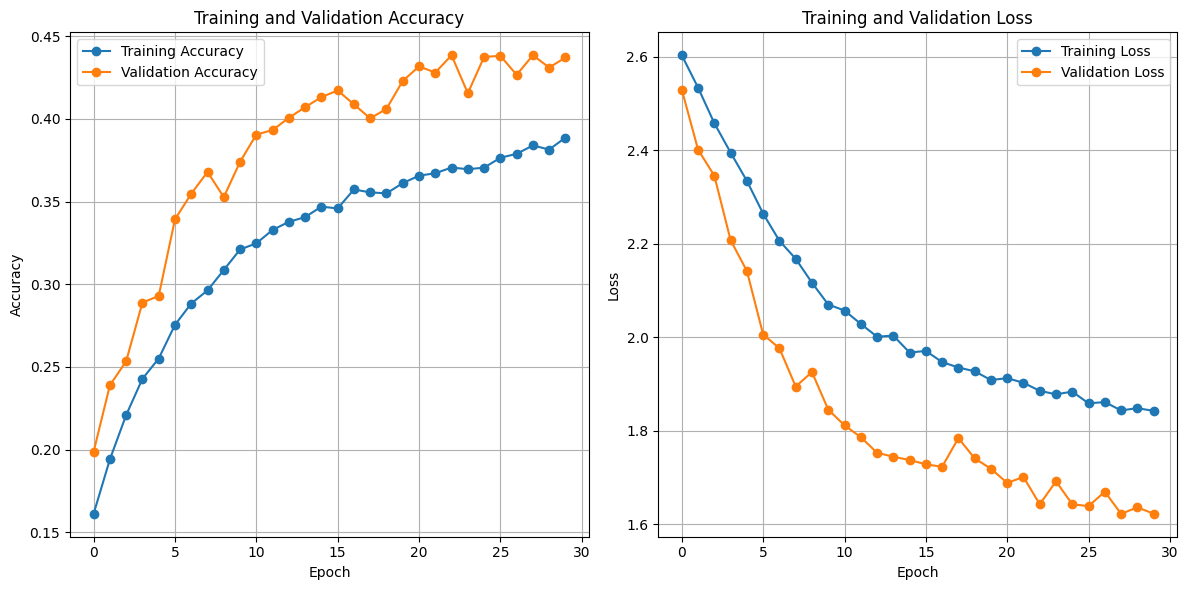
\includegraphics[width=\textwidth]{assets/confusion_matrix/grayscale/CNN_history.png}
        \caption{CNN training history}
    \end{subfigure}
    \caption{Taining history for MLP and CNN models (grayscale)}
    \label{fig:grayscale_training_history}
\end{figure}


\FloatBarrier 
\newpage
\subsection{RGB scores}
\subsubsection{RGB Model Training and Testing Accuracy}
Table \ref{tab:RGB scores} summarizes the accuracy results of different models on the dataset using RGB image. (we dont add a Note column because the results are similar to the grayscale image)

\begin{table}[htbp]
    \centering
    \begin{tabular}{lcc}
        \toprule
        Model & Train Accuracy & Test Accuracy \\
        \toprule
        Softmax & 0.7331 & 0.3237 \\
        \midrule
        SVM & 0.2045 & 0.1751 \\
        \midrule
        Random Forest & 0.7728 & 0.3218 \\
        \midrule
        AdaBoost & 0.3716 & 0.3162 \\
        \midrule
        K-NN (k=1) & 0.9998 & 0.1917 \\
        \midrule
        K-NN (k=3) & 0.7778 & 0.2092 \\
        \midrule
        K-NN (k=7) & 0.6886 & 0.2279 \\
        \midrule
        K-NN (k=9) & 0.6658 & 0.2333 \\
        \midrule
        MLP & 0.7950 & 0.3478 \\
        \midrule
        CNN & 0.4718 & 0.3298 \\
        \bottomrule
    \end{tabular}
    \caption{Train and Test Accuracy of Various Models with RGB image}
    \label{tab:RGB scores}
\end{table}
\FloatBarrier 

\subsubsection{RGB Model Confusion Matrices}
Here are confusion matrices for rgb models, they show where model predictions are right (on diagonal) and where they are wrong (not on diagonal).

\begin{figure}[H]
    \centering
    \begin{subfigure}[b]{0.48\textwidth}
        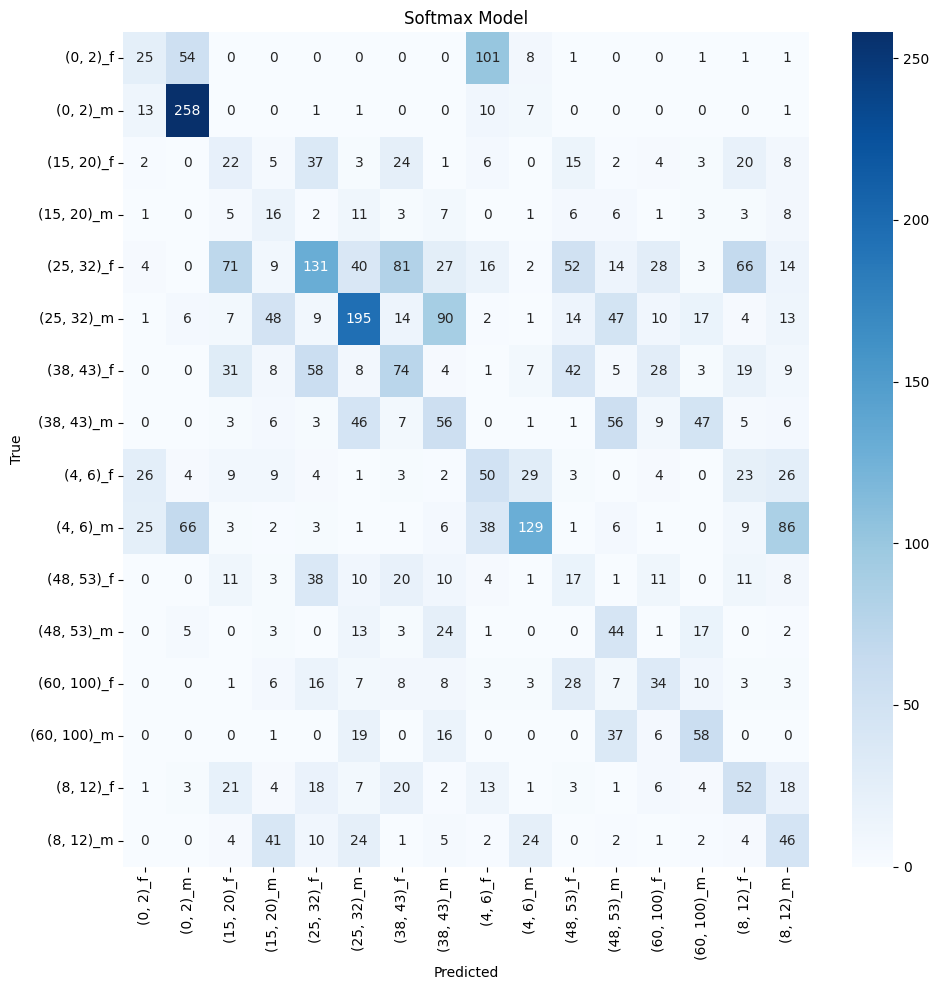
\includegraphics[width=\textwidth]{assets/confusion_matrix/rgb/Softmax Model.png}
        \caption{Softmax}
    \end{subfigure}
    \hfill
    \begin{subfigure}[b]{0.48\textwidth}
        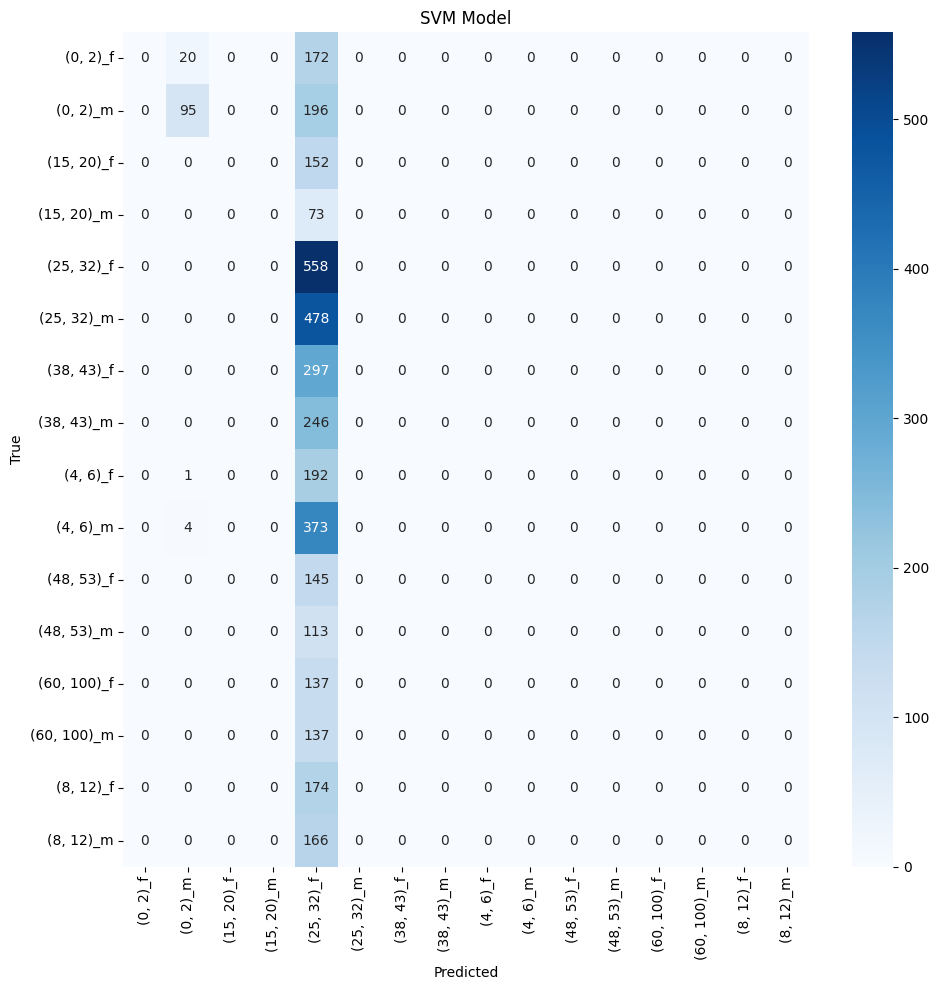
\includegraphics[width=\textwidth]{assets/confusion_matrix/rgb/SVM Model.png}
        \caption{SVM}
    \end{subfigure}
    \caption{Confusion matrices for Softmax and SVM models (rgb)}
    \label{fig:rgb_confusion_matrices_1}
\end{figure}

\begin{figure}[H]
    \centering
    \begin{subfigure}[b]{0.48\textwidth}
        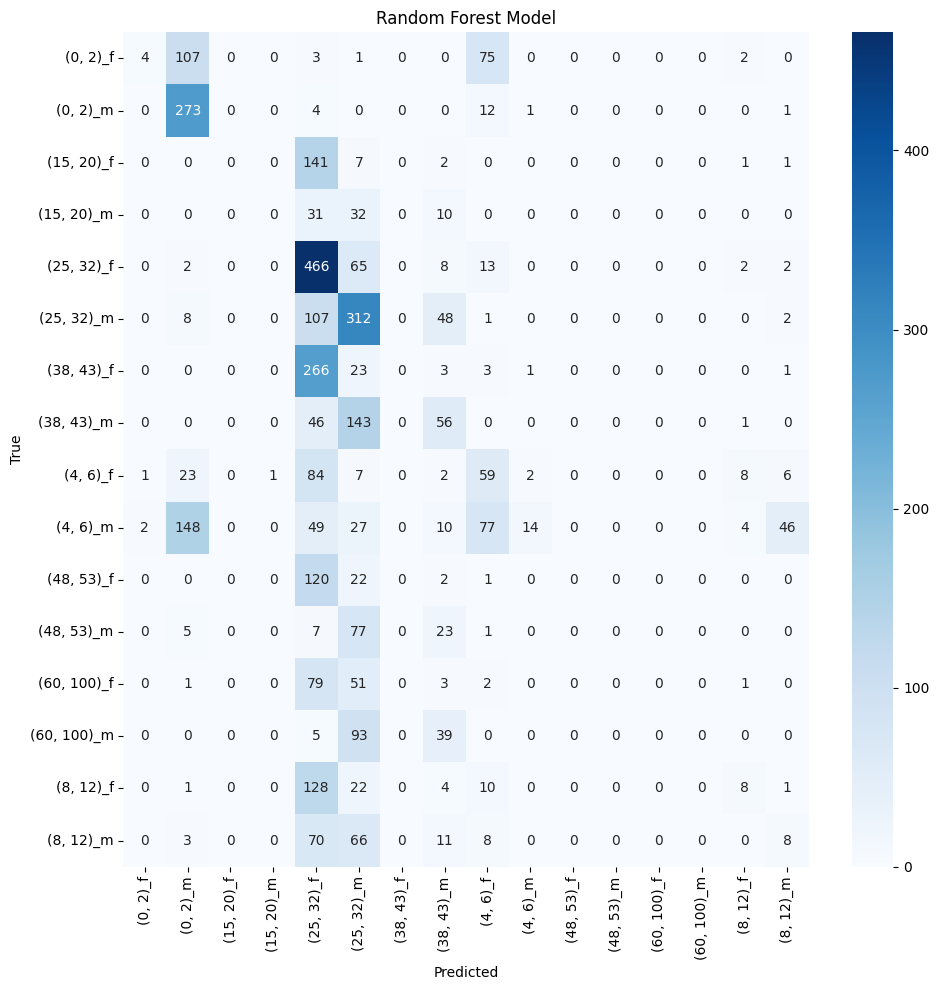
\includegraphics[width=\textwidth]{assets/confusion_matrix/rgb/RF Model.png}
        \caption{Random Forest}
    \end{subfigure}
    \hfill
    \begin{subfigure}[b]{0.48\textwidth}
        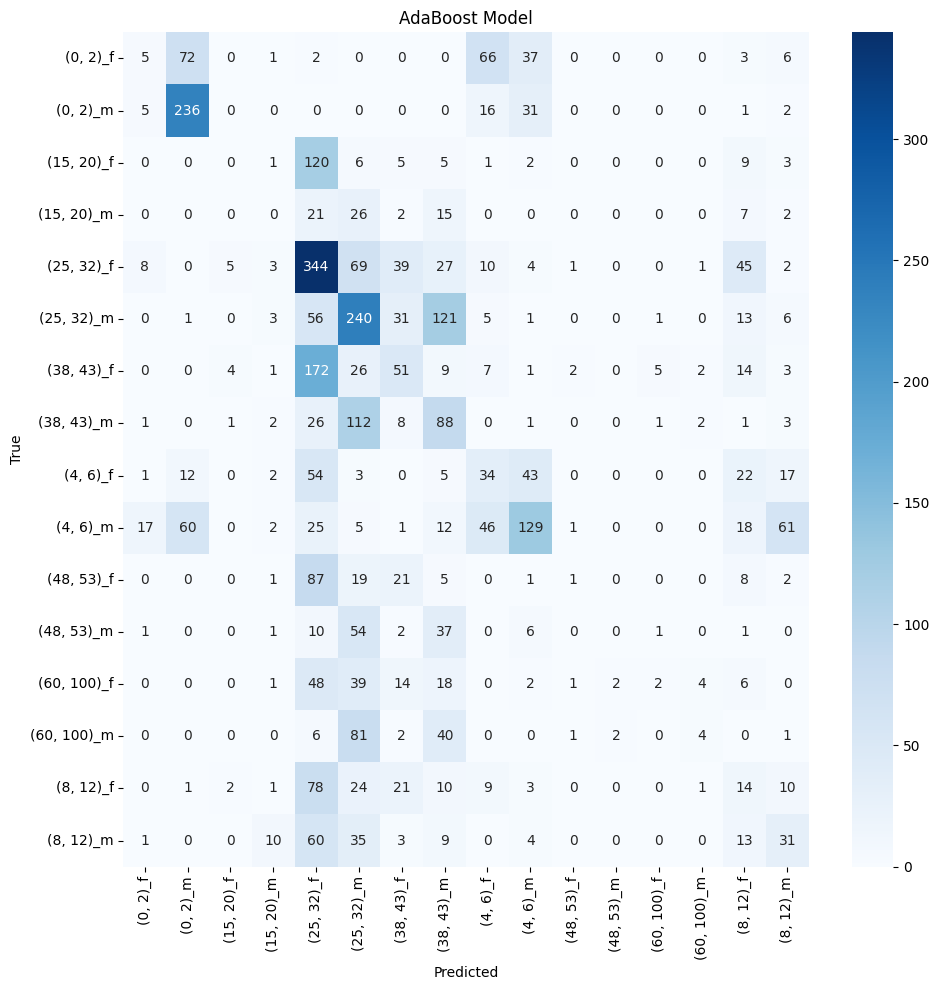
\includegraphics[width=\textwidth]{assets/confusion_matrix/rgb/AdaBoost Model.png}
        \caption{AdaBoost}
    \end{subfigure}
    \caption{Confusion matrices for Random Forest and AdaBoost models (rgb)}
    \label{fig:rgb_confusion_matrices_2}
\end{figure}

\begin{figure}[H]
    \centering
    \begin{subfigure}[b]{0.48\textwidth}
        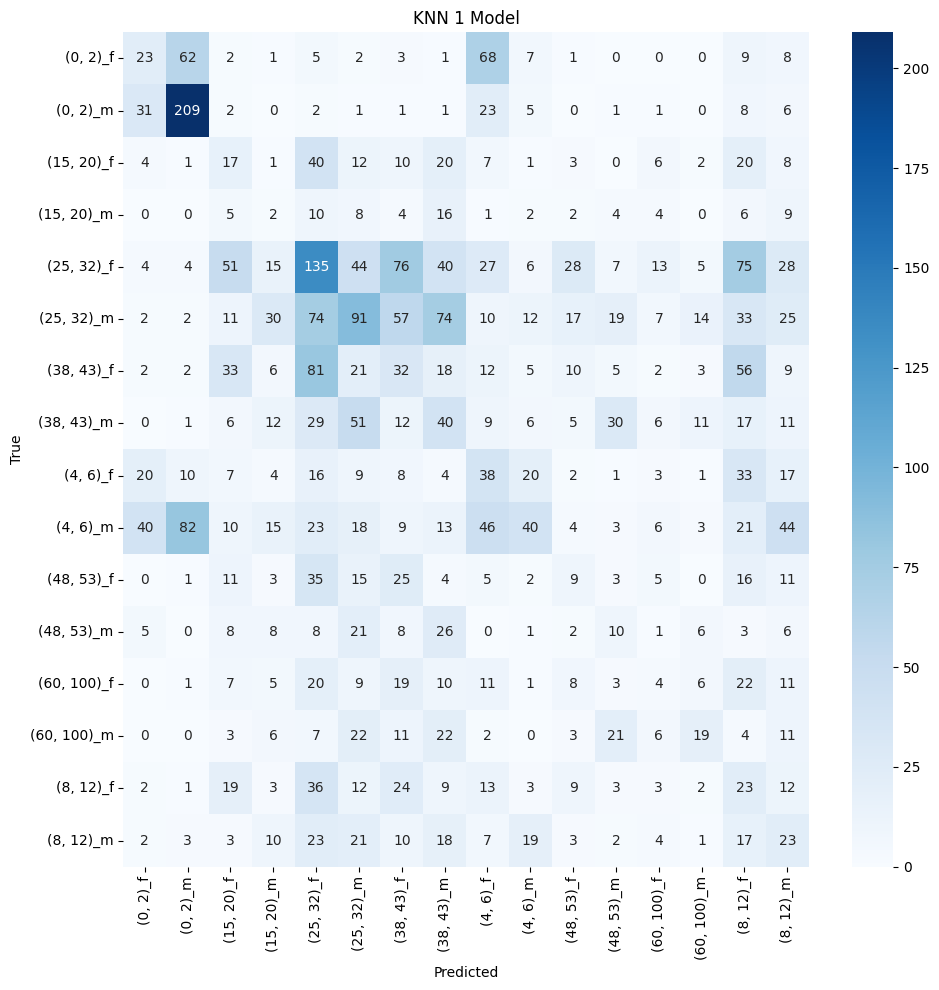
\includegraphics[width=\textwidth]{assets/confusion_matrix/rgb/KNN1.png}
        \caption{KNN (k=1)}
    \end{subfigure}
    \hfill
    \begin{subfigure}[b]{0.48\textwidth}
        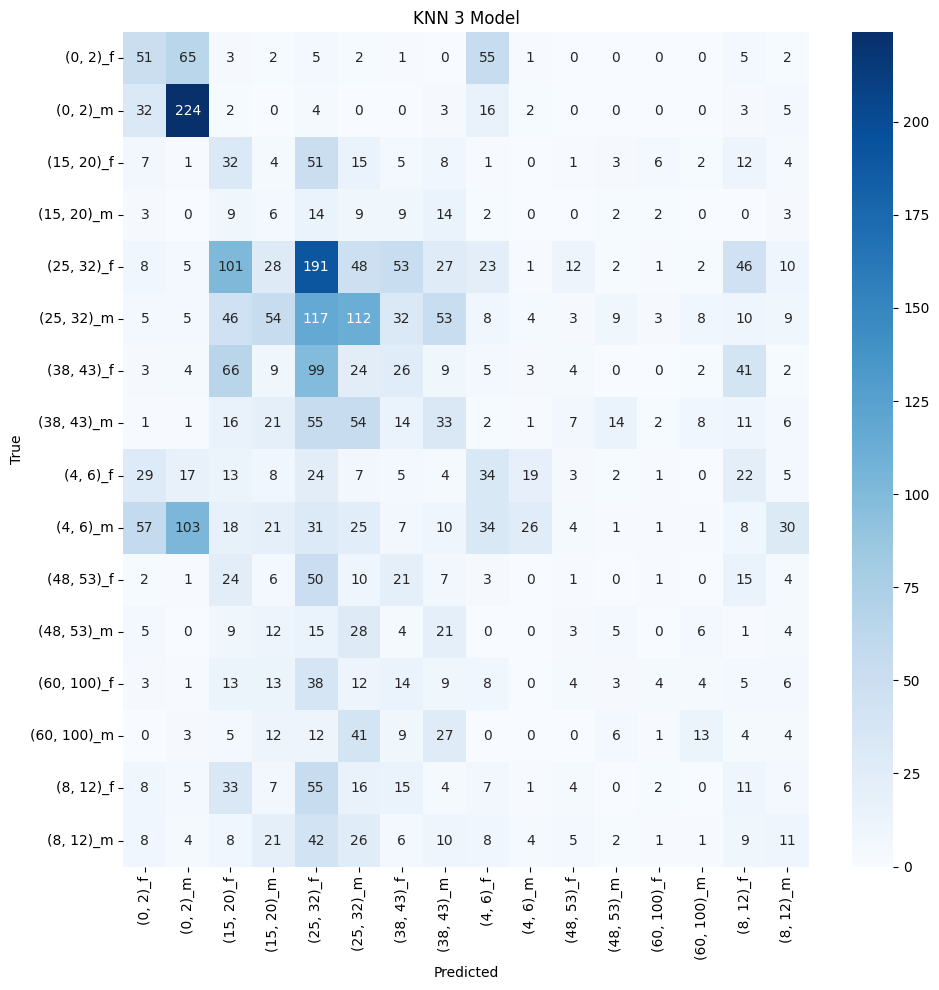
\includegraphics[width=\textwidth]{assets/confusion_matrix/rgb/KNN3.png}
        \caption{KNN (k=3)}
    \end{subfigure}
    \caption{Confusion matrices for KNN models with k=1 and k=3 (rgb)}
    \label{fig:rgb_confusion_matrices_3}
\end{figure}

\begin{figure}[H]
    \centering
    \begin{subfigure}[b]{0.48\textwidth}
        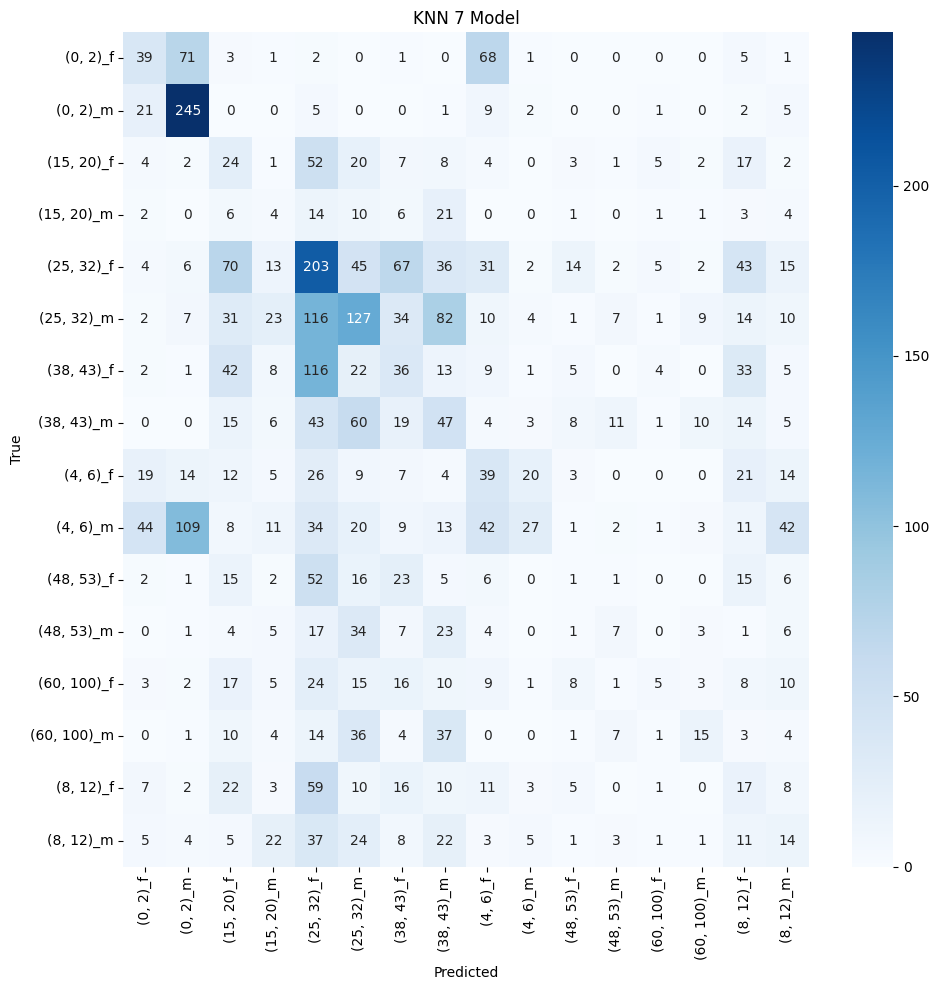
\includegraphics[width=\textwidth]{assets/confusion_matrix/rgb/KNN7.png}
        \caption{KNN (k=7)}
    \end{subfigure}
    \hfill
    \begin{subfigure}[b]{0.48\textwidth}
        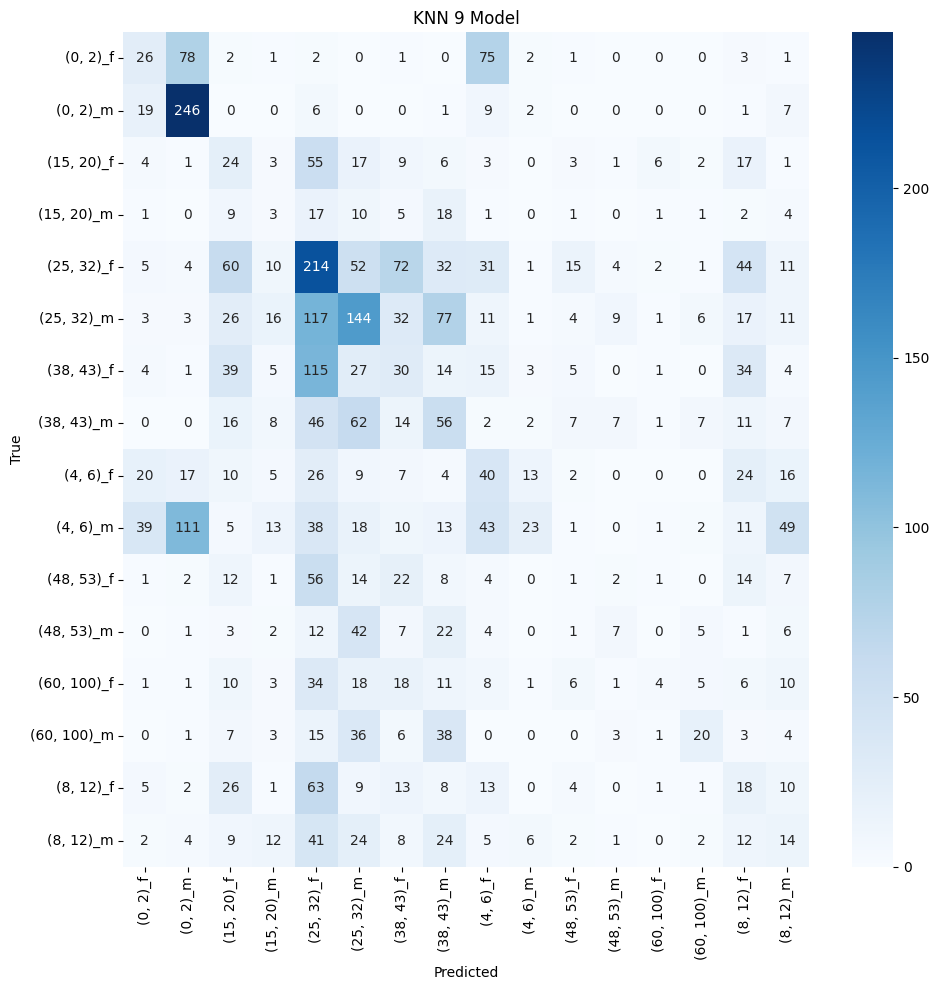
\includegraphics[width=\textwidth]{assets/confusion_matrix/rgb/KNN9.png}
        \caption{KNN (k=9)}
    \end{subfigure}
    \caption{Confusion matrices for KNN models with k=7 and k=9 (rgb)}
    \label{fig:rgb_confusion_matrices_4}
\end{figure}

\begin{figure}[H]
    \centering
    \begin{subfigure}[b]{0.48\textwidth}
        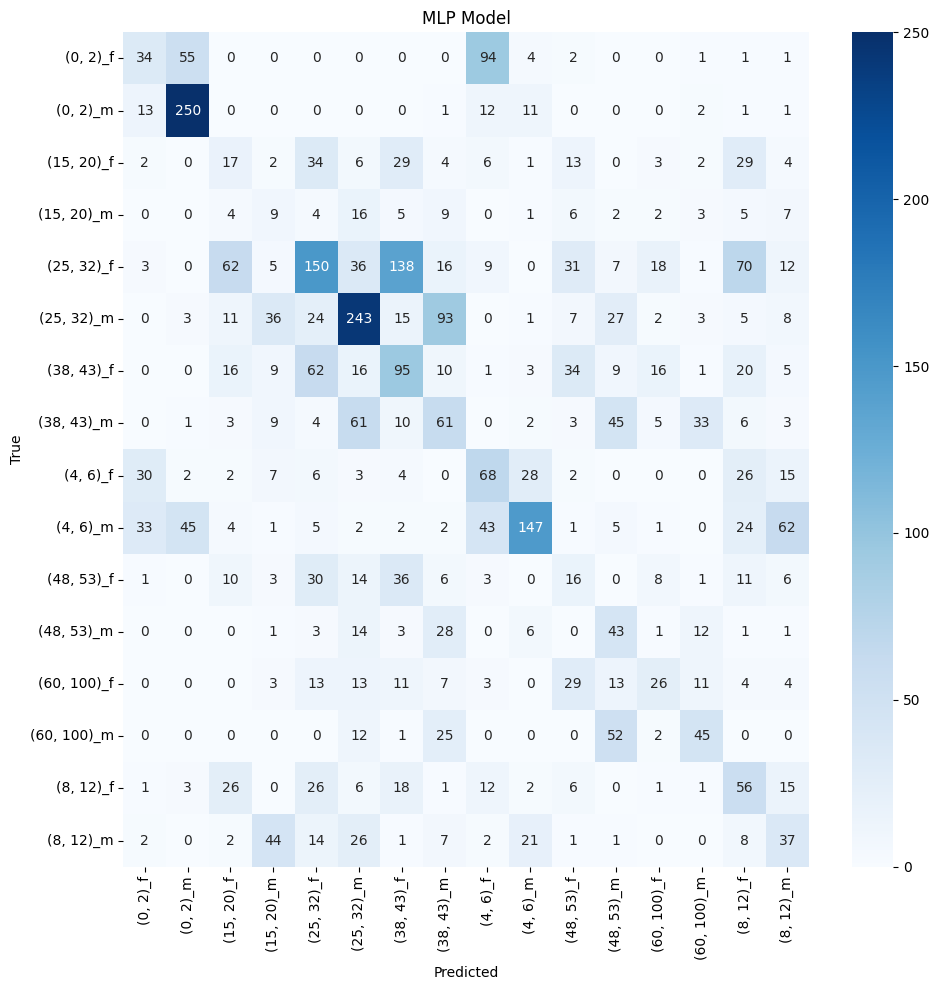
\includegraphics[width=\textwidth]{assets/confusion_matrix/rgb/MLP.png}
        \caption{MLP}
    \end{subfigure}
    \hfill
    \begin{subfigure}[b]{0.48\textwidth}
        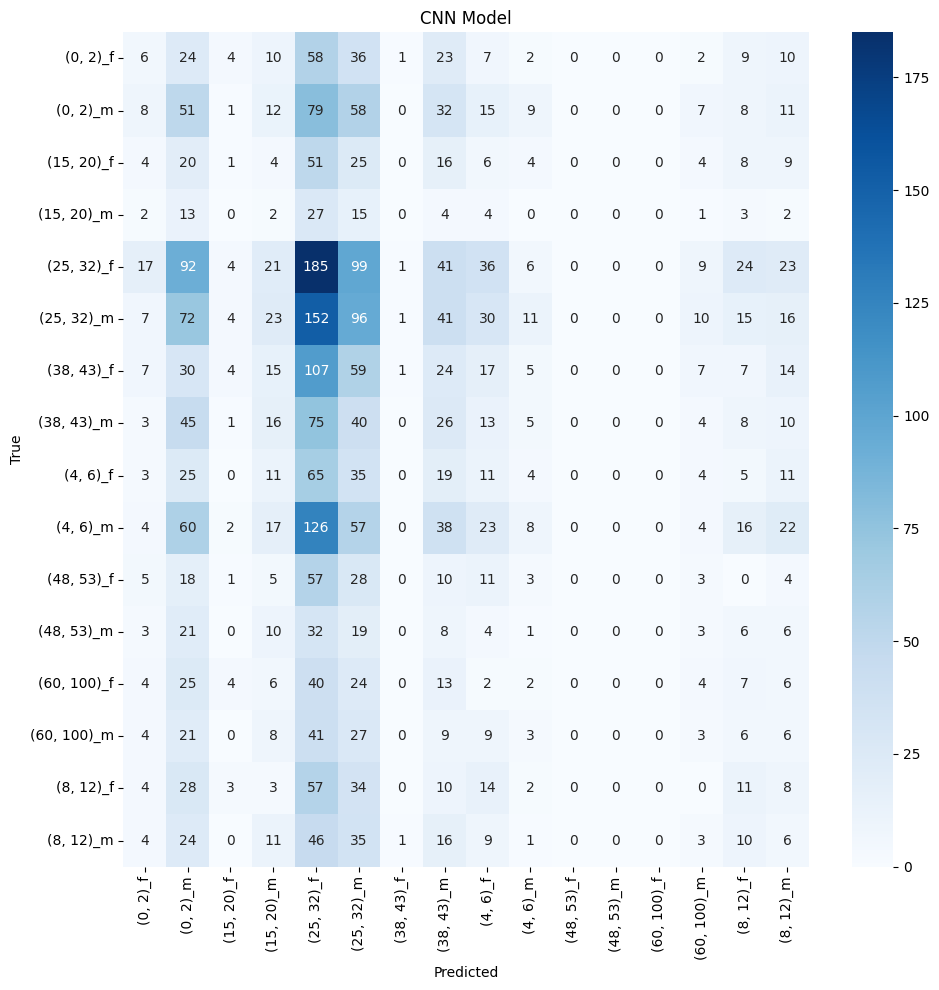
\includegraphics[width=\textwidth]{assets/confusion_matrix/rgb/CNN.png}
        \caption{CNN}
    \end{subfigure}
    \caption{Confusion matrices for MLP and CNN models (rgb)}
    \label{fig:rgb_confusion_matrices_5}
\end{figure}

\begin{figure}[H]
    \centering
    \begin{subfigure}[b]{0.48\textwidth}
        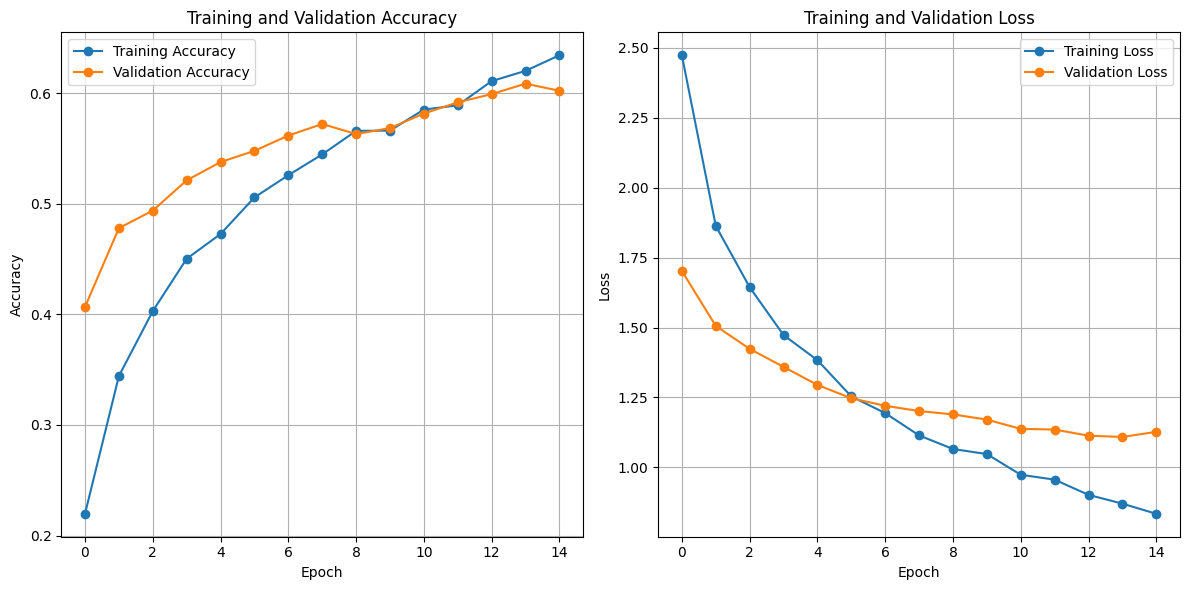
\includegraphics[width=\textwidth]{assets/confusion_matrix/rgb/MLP_history.png}
        \caption{MLP training history}
    \end{subfigure}
    \hfill
    \begin{subfigure}[b]{0.48\textwidth}
        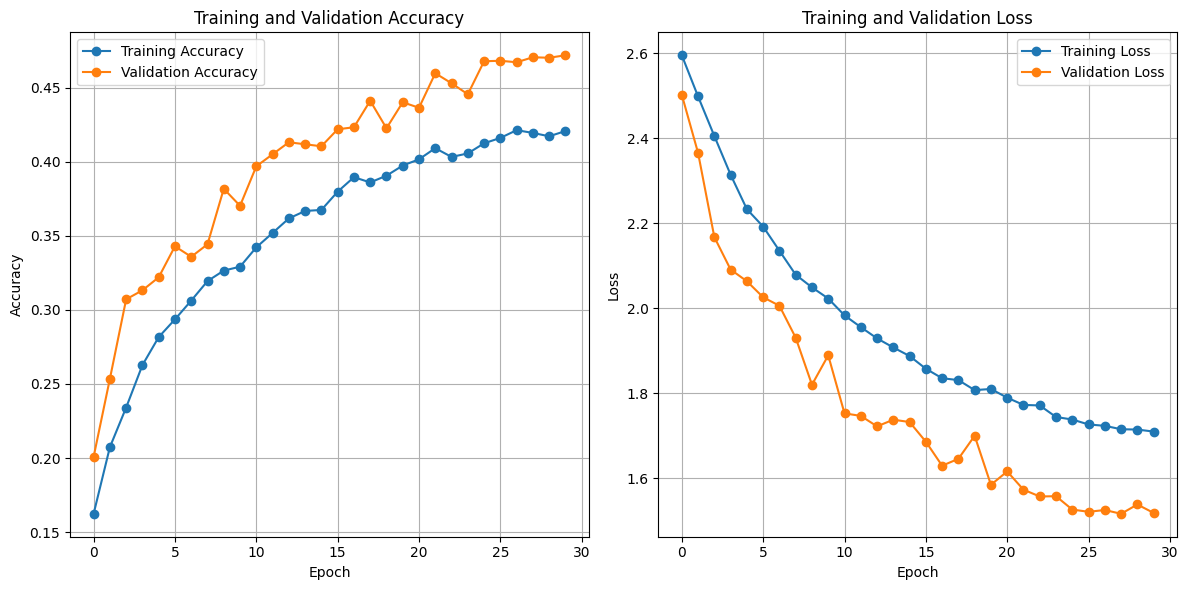
\includegraphics[width=\textwidth]{assets/confusion_matrix/rgb/CNN_history.png}
        \caption{CNN training history}
    \end{subfigure}
    \caption{Taining history for MLP and CNN models (rgb)}
    \label{fig:rgb_training_history}
\end{figure}
\newpage
\subsection{Analysis of Results}

Our results show important patterns across different models and processing methods. Here we analyze what we found.

\subsubsection{General Performance Trends}

We see that models trained on RGB features perform little better than grayscale ones, which mean color information helps for age and gender classification. The best model was MLP with RGB features (34.78\% test accuracy), and worst was SVM (17.51\% test accuracy on RGB).

The test accuracies (17.51\% to 34.78\%) are not very high because this is hard task with 16 classes (age+gender). Random guessing would give about 6.25\% accuracy, so our models are 3-5 times better than random.

\subsubsection{Model-Specific Analysis}

\paragraph{Softmax Regression:} 
Softmax got good performance (32.37\% test accuracy with RGB) even though it is simple model. This mean our feature space have some linear separability. The confusion matrix show it was best on big classes like (0, 2)\_m and (25, 32)\_m, with most errors between close age groups not gender mistakes.

\paragraph{Support Vector Machine (SVM):}
SVM perform badly (17.51\% test accuracy), which suggest the high-dimensional feature space was not good for finding hyperplanes. SVM mostly predict the (25, 32)\_f class—our biggest class—showing it bias toward majority classes even with class weighting.

\paragraph{Random Forest:}
Random Forest perform well (32.18\% test accuracy with RGB), showing it can catch complex patterns with many decision trees. The model learn feature importance patterns from ResNet50 embeddings, and depth-limited trees (max\_depth=10) help control overfitting. But like other models, it have trouble with small classes.

\paragraph{AdaBoost:}
AdaBoost show medium performance (31.62\% with RGB), focusing on hard-to-classify examples. This work well for our imbalanced dataset, and we see smaller gap between train and test accuracy compared to Random Forest.

\paragraph{K-Nearest Neighbors (KNN):}
KNN show clear overfitting, especially with small k. With k=1, model got almost perfect training accuracy (99.98\%) but bad test performance (19.17%), which mean it just "memorize" data not generalize. As k get bigger, both overfitting and accuracy go down, with k=9 showing best test performance among KNN models. This show that more neighbors voting help smooth decision boundaries in high-dimensional spaces.

\paragraph{Multi-Layer Perceptron (MLP):}
MLP got best performance (34.78\% test accuracy with RGB), showing deep learning better for complex patterns. The dense layers with dropout (0.5) and batch normalization control overfitting while keeping good representation. Early stopping also help generalization by stopping training at right time.

\paragraph{Convolutional Neural Network (CNN):}
CNN perform well (32.98\% with RGB) even when trained on raw images not extracted features. This show end-to-end learning can be good as transfer learning for this task. The smaller gap between training (47.18\%) and testing (32.98\%) accuracy suggest CNN architecture have some natural regularization compared to other models.

\subsubsection{Overfitting Analysis}

All models had some overfitting, we see in gap between training and test accuracy. This happen because:

\begin{itemize}
    \item \textbf{Limited data diversity:} Even with thousands of images, we don't have enough samples per class for good generalization across all 16 classes.
    
    \item \textbf{Class imbalance:} The uneven distribution of samples across age and gender categories make it hard for models to learn good representations of small classes.
    
    \item \textbf{High-dimensional feature space:} The 2048-dimensional ResNet50 features create very big feature space compared to training examples, which make overfitting more likely.
\end{itemize}

\subsubsection{RGB vs. Grayscale Performance}

RGB models always perform better than grayscale, but not by much (usually 1-3 percentage points). This mean color information is helpful but not essential for age-gender classification. Color information maybe help with things like skin tone changes with age or makeup differences between genders.

\subsubsection{Error Pattern Analysis}

Confusion matrices show consistent error patterns in all models:

\begin{itemize}
    \item Most wrong predictions happen between close age groups (like (25, 32) and (38, 43)), which show it hard to put ages in exact groups based only on face features.
    
    \item Gender mistakes happen less than age group mistakes, which mean gender features are more clear than age features in face images.
    
    \item Some age-gender combinations, especially ones with few training examples, always get poor classification results in all models.
\end{itemize}

This analysis show that while our models give useful age-gender classification, there is still lot of room for improvement with better architectures, data augmentation, and training strategies for this multi-class problem.

\newpage
\section{Research Questions}

\subsection*{Question 1: Different Types of People}
\begin{itemize}[leftmargin=1.6cm]
    \item Does it work the same for people from different places?
    \item Can we use the same model everywhere or do we need different ones?
\end{itemize}
\subsection*{Answer to Question 1}  
To explore these questions, we used the UTKFace dataset \cite{UTKFace_dataset}, which contains images of people from diverse ethnic backgrounds with labeled age, gender, and ethnicity information. 
Our analysis aimed to determine whether the model performs consistently between different groups.

\begin{enumerate}
    \item \textbf{Image Path Construction}: Image paths were constructed to facilitate loading - the dataset was diffrent, and the way that we ajust the data to work with our model can see in \href{https://github.com/ShayGali/VisAge/blob/main/questions/q1.ipynb}{q1.ipynb}.
    \item \textbf{Label Encoding}: Age and gender were combined and encoded for model training.
\end{enumerate}

A pie chart of race distribution illustrates the diversity within the dataset. Age and gender distributions were plotted for each racial group to provide context for analysis.

Multiple models, including CNNs and various machine learning models, were loaded for evaluation:
\begin{itemize}
    \item \textbf{CNN Models}: Trained on RGB images and grayscale images.
    \item \textbf{Sklearn Models}: Includes classifiers like AdaBoost, KNN, Random Forest, Softmax, and SVM.
\end{itemize}

Preprocessing of both RGB and grayscale images was performed. Features were stored in \texttt{.npy} files to prevent redundant processing.

Models were evaluated across different racial groups, with results summarized as follows:

\textbf{Model Accuracy by Race}
\begin{table}[H]
    \centering
    \renewcommand{\arraystretch}{1.2}
    \begin{tabular}{|c|c|c|c|c|c|}
    \hline
    \textbf{Model} & \textbf{White} & \textbf{Black} & \textbf{Asian} & \textbf{Indian} & \textbf{Other} \\
    \hline
    CNN & 0.17 & 0.11 & 0.17 & 0.14 & 0.22 \\
    \hline
    AdaBoost & 0.18 & 0.13 & 0.17 & 0.15 & 0.20 \\
    \hline
    KNN & 0.17 & 0.15 & 0.19 & 0.14 & 0.17 \\
    \hline
    Random Forest & 0.19 & 0.17 & 0.20 & 0.17 & 0.23 \\
    \hline
    Softmax & 0.23 & 0.18 & 0.25 & 0.22 & 0.23 \\
    \hline
    SVM & 0.07 & 0.07 & 0.07 & 0.06 & 0.08 \\
    \hline
    \end{tabular}
    \caption{Model accuracy across different racial groups.}
    \label{tab:accuracy_race}
\end{table}

The accuracy rates suggest variability in model performance across different races, which could indicate biases in model training or dataset representation. Models tended to perform better on the "Other" category, suggesting that there is a more even distribution of features in this group, or it could be less represented in some training aspects. But we can see that the prediction on "Black" was the worst, which could indicate that the model was not trained well on this group.


\subsection*{Question 2: Can We Use This in Real Life?}
\begin{itemize}[leftmargin=1.6cm]
    \item Will it work fast enough for apps or security cameras?
    \item What about when there is bad lighting or people wear glasses?
\end{itemize}

\subsection*{Answer Question 2}
To evaluate real-time performance, we built a face recognition system that detects age and gender when people appear in front of the camera.
Our results show that most models perform well in real-time scenarios, even with poor lighting or glasses, making it suitable for applications such as mobile applications and security cameras.  
\\ Just one model - the SVM - showed a significant decrease in performance in real-time scenarios, indicating that it may not be suitable for such applications.
 


\subsection*{Question 3: About Age and gender prediction}
\begin{itemize}[leftmargin=1.6cm]
    \item Which model is best at dealing with different age and gender?
    
\end{itemize}

\subsection*{Answer to Question 3}
From the analysis of the models, we can see that the model with the less overfitting, 
and when the model got wrong predictions, it was not by much (the most of the error in the confusion matrix was in the adjacent age group), it was the MLP model.

\subsection*{Question 4: How Models Work with Different Images}
\begin{itemize}[leftmargin=1.6cm]
    \item What happens when images are not clear or blurry?
    \item Do facial expressions (such as smiling or not smiling) affect the results?
\end{itemize}

\subsection*{Answer Question 4}
To investigate the impact of facial expressions on the predictions of the model,
we examined four different emotional states: smiling, serious, mad and regular. 
Our analysis revealed that all models produced consistent predictions in these expressions,
indicating that facial expressions do not significantly influence the results.\\
Also from the real-time analysis, we can see that the model works well with different images, even with blurry images, which makes it suitable for real-world applications.


\newpage
\section{Challenges in Gender and Age Classification using Adience Benchmark Dataset}
\subsection{Data Structure and Organization Challenges}
When we explore the Adience Benchmark dataset, we find several structure problems:

\begin{itemize}
    \item \textbf{Duplicate folders:} The dataset have two \texttt{faces} folders with same content, so we need to check which folder to use without losing important data.

    \item \textbf{Files in many places:} Files were spread in many different fold directories, so we need special code to combine all dataset together.

    \item \textbf{Keeping people separate:} We need to make sure images from same person don't appear in both training and testing sets by checking the \texttt{user\_id} across different folds.
\end{itemize}

\subsection{Data Quality and Preprocessing Challenges}
The dataset have many quality and preprocessing problems we need to fix:

\begin{itemize}
    \item \textbf{Age labels not consistent:} Some labels have specific ages (like '22', '35', '58') and some have age ranges (like '(0, 2)', '(25, 32)'), so we need process to put single ages into right ranges.

    \item \textbf{Age ranges that overlap:} We find many overlapping age groups:
    \begin{itemize}
        \item Same range with different numbers: (38, 42), (38, 43), and (38, 48)
        \item Similar ranges with different start/end: (25, 32) and (27, 32)
        \item Ranges that don't make sense together: (8, 12), (8, 23), and (15, 20)
    \end{itemize}

    \item \textbf{Missing gender labels:} Many images (especially in (0, 2) age range) have 'u' for gender, so we need to remove them or guess gender.

    \item \textbf{Missing data:} Some records have NaN values that we need to handle by filling in values or removing them.
\end{itemize}

\subsection{Class Imbalance Challenges}
When we check the dataset, we find big problems with balance:

\begin{itemize}
    \item \textbf{Age groups not equal:} The (25, 32) age range had too many samples (5391), but other ranges like (60, 100) had very few (just 896).

    \item \textbf{Gender not balanced:} In some age groups, one gender has much more samples than other gender.

    \item \textbf{Unknown gender problem:} Most images with 'u' gender label were in (0, 2) age range, this make bias in the data.
\end{itemize}

\subsection{Feature Engineering and Extraction Challenges}
When we try to convert images to features, we face many problems:

\begin{itemize}
    \item \textbf{ResNet50 is too big:} Using ResNet50 need a lot of computer power and we need to optimize it for our task.

    \item \textbf{Features too many or too few:} It's hard to decide how many features from ResNet50 is good - too many make slow model, too few lose information.
\end{itemize}

\subsection{Early Stopping Problems}
When we try to use early stopping to stop overfitting, we face many challenges:

\begin{itemize}
    \item \textbf{Which metric to check:} Hard to choose right metrics to watch:
    \begin{itemize}
        \item Should we watch both age and gender accuracy or just one?
        \item Sometimes loss goes down but accuracy not improve
        \item Not sure if we need special metrics for imbalanced classes
    \end{itemize}

    \item \textbf{Patience value problem:} Hard to choose how many epochs to wait before stopping:
    \begin{itemize}
        \item Too little waiting: Might stop too early before model learn good weights
        \item Too much waiting: Waste time and might overfit
    \end{itemize}

    \item \textbf{Learning rate changes:} Hard to use with learning rate scheduler:
    \begin{itemize}
        \item Not sure if model stuck or just need learning rate change
        \item Should we reset patience after change learning rate?
    \end{itemize}

    \item \textbf{Saving models:} Need to decide about checkpoints:
    \begin{itemize}
        \item Need lot of disk space to save models during training
        \item Not sure if save model with best validation loss or best accuracy
        \item How to load best model when training finish
    \end{itemize}

    \item \textbf{Planning compute time:} Hard to know how long training will take:
    \begin{itemize}
        \item Different models stop at different times
        \item Need balance between trying many parameters and saving time
    \end{itemize}
\end{itemize}

\subsection{Combined Age-Gender Prediction Problems}
Predicting both age and gender together was hard:

\begin{itemize}
    \item \textbf{How to setup problem:} We need to decide:
    \begin{itemize}
        \item Make two separate models (one for age, one for gender)
        \item Make one model that predicts combined age-gender classes
        \item Make one model with shared features but separate outputs
        \item From our observation, the method that work the best for us was to make one model that predicts in combined lable.
    \end{itemize}



    \item \textbf{Loss function problems:} Hard to balance how much age errors and gender errors matter.

    \item \textbf{Evaluating results:} Need special way to measure if model good at both age and gender.
\end{itemize}

\subsection{Training and Testing Split Problems}
Making good train and test splits had many problems:

\begin{itemize}
    \item \textbf{How to split data:} Dataset already had folds, but we need validation set too.

    \item \textbf{No data leaking:} Need make sure same person not in both train and test set.

    \item \textbf{Keeping fold info:} Need track which images come from which original folds.
\end{itemize}


\newpage
\section{Real time application}
We make camera application that can detect faces and predict age and gender in real time.
We use our best model - MLP with RGB features - for this app.
\\
We build this app with OpenCV for finding faces, TensorFlow for running our model, and Tkinter for making simple window interface.
\\
\subsection{How the app works}

\begin{itemize}
    \item The app open window that show live video from camera.
    \item When app see face in video, it predict age and gender. We make prediction every 3 frames to save computer power.
    \item App show age range and gender on top of each face, also show how confident model is about prediction.
    
\end{itemize}

\subsection{Image of the app}
\begin{figure}[H]
    \centering
    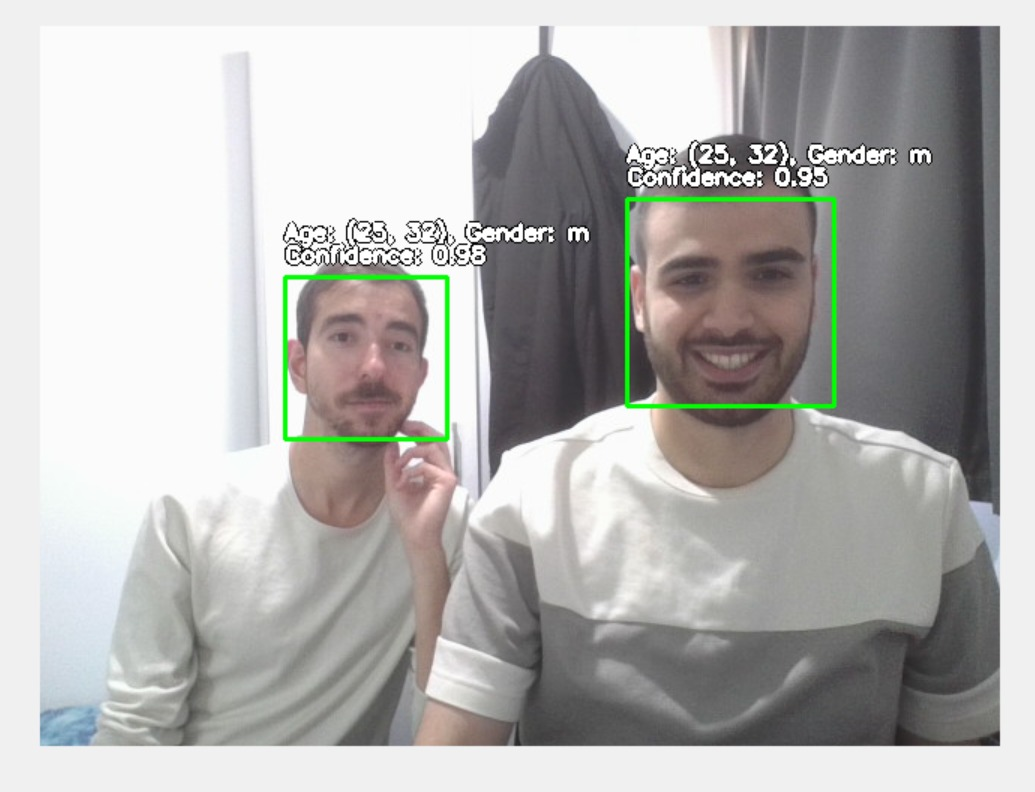
\includegraphics[width=0.8\textwidth]{assets/app.jpg}
    \caption{Real-time Age and Gender Prediction App}
    \label{fig:app}
\end{figure}

\printbibliography

\end{document}
